\documentclass[12pt,a4paper]{article}
\usepackage[utf8]{inputenc}
\usepackage{amsmath,esint}
\usepackage{amsfonts}
\usepackage{amssymb}
\usepackage{geometry}
\usepackage{setspace}
\doublespacing
\usepackage{graphicx}
\usepackage{float}
\usepackage{wrapfig}
\usepackage{caption}
\usepackage{sidecap}
\usepackage{subcaption}
\usepackage{tabulary}
\usepackage{pdflscape}
\usepackage{afterpage}
\usepackage{capt-of}% or use the larger `caption` package
\usepackage[usenames, dvipsnames]{color}
\usepackage{lineno}
\linenumbers*[1]
\usepackage{enumitem}
\newlist{arrowlist}{itemize}{1}
\setlist[arrowlist]{label=$\Rightarrow$}
\usepackage{cite}


\author{Kelian Dascher-Cousineau}
\title{Masters Thesis: The Evolution of Fault Slip Surfaces with Cumulative Displacement}


\begin{document}

\maketitle

\printbibliography

\begin{abstract}

Fault slip surface roughness determines fault strength, friction and dynamic fault processes. Wear models and field observations suggest that roughness decreases with cumulative displacement. However, measurements have yet to isolate the effect of displacement from other possible controls, such as lithology or tectonic setting. We present an unprecedentedly large fault surface dataset collected in and around the San-Rafael Desert, S.E. Utah, United States. In the study area, faults accommodated regional extension at shallow 1 to 3 $km$ depth and are hosted in the massive, well sorted, high porosity Navajo and Entrada sandstones. Existing detailed stratigraphic throw profile provide a maximum constraint for displacement. Where cross-sectional exposure is good, we measure exact displacement imparted on slip surfaces using offset in marker horizons. Thereby, we isolate for the effect of displacement during the embryonic stages of faulting (0 to 60 $m$ in displacement). Our field observations indicate a clear compositional and morphological progression from isolated joints or deformation bands towards smooth, continuous and mirror-like fault slip surfaces with increasing displacement. To quantify these observations, slip surfaces were scanned with a white light interferometer, a laser scanner and a ground based Lidar. Together these instruments resolve more than eight decades of spatial bandwidth (from less than $\mu m$'s to $m$'s in scale). Results indicate that roughness as defined by the power ($P$) at a given wavelength ($\lambda$) decreases with displacement ($D$) according to a power law, $P(\lambda) \varpropto D^{0.6 \pm 0.1}$. Trends are however subject to significant scatter. Roughness measurement associated with only maximum constraints on displacements corroborate this result—for a given displacement, minimum roughness is bounded by the later smoothing trend. In addition, we find that the maximum roughness is fixed—bounded a by a primordial roughness corresponding to that of joints surfaces and deformation band edges. Building upon our results, we propose a wear model to explain the evolution of faults with displacement. The basis of the model is supported by numerical simulations of crack initiation and growth using boundary element models Fri2D and growth by work-minimization (GROW). Our modelling provides the first insight into fault slip surface process consistent with observational constraints, i.e. fractal geometry and a nearly power-law decay with displacement, by using calling upon scale dependent strength, strength heterogeneity and scale invariant asperity failure by truncation.

\end{abstract}

\section*{Contribution of Authors}

\section{Introduction}

Faults are a characteristic feature of the Earth’s brittle crust. Fluid flow, seismicity and crustal mineralization are just few systems upon which faults act as major controls \cite{sibson1977fault} (more citations...). In spite of their importance, some aspects of faults and their underlying processes remain poorly understood. How strong is a fault? How do faults mature? Are small faults mechanically different to large faults? Fault geometry has been shown to be a key parameter controlling the mechanical behavior and evolution of faults (e.g. \cite{lay1982asperity} \cite{aki1984asperities} \cite{power1988roughness} \cite{chester2000stress}), but these questions are not yet fully answered.

Slip on a fault occurs on discrete slip surfaces in fault zones \cite{davatzes2005distribution}. These surfaces are not planar; they are rough. Roughness is observable at all scales \cite{scholz1986fractal} \cite{candela2011fault}. Slickenlines, corrugations, mullions and jogs are all  surface features that can be seen at different length scales \cite{sagy2009geometric}. Field studies have found common characteristics in the topography of fault surfaces. These can be summarized as follows: 1) Fault surfaces appear to be well defined by large fractal domains, wherein 2) faults are smoother at larger length scales \cite{scholz1986fractal} \cite{candela2011fault}, 3) rougher in the slip perpendicular direction than in the slip parallel direction \cite{lee1996structural} and 4) slip surfaces are smoother with cumulative displacement \cite{sagy2007geometric}\cite{brodsky2011faults}. Fault roughness has been demonstrated to be critical in determining the strength \cite{chester2000stress} \cite{brodsky2016constraints}, triggering \cite{parsons2008persistent}, dynamic properties \cite{candela2011stress}; Dunham et al., 2011), spatial distribution (Parson, 2008) and failure recurrence of faults (Stirling et al., 1996). It is increasingly evident that roughness is a fingerprint of fundamental features of the faulting process \cite{brodsky2016constraints} \cite{candela2011stress}. In accordance, incorporating more complex sources geometries has become a more frequent practice in dynamic earthquake rupture modelling \cite{shi2013rupture} . 

Changes in roughness, as determined by cumulative displacement (Sagy et al, 2007; Brodsky et al, 2011), imply faults mature. Fundamental differences between immature and mature fault have far-reaching implications. Fixed source parameter scaling of earthquakes is a pillar of earthquake seismology. However, analysis of seismic signals of immature faults vs. mature faults suggest that scaling is sensitive to cumulative displacement. This observation leads to an interpretation of fundamental differences in earthquake populations. Specifically fault maturation would undermine the applicability of a constant magnitude scaling. Evolving mechanical properties such as fault friction and static strength—both associated to fault roughness—would imply that immature and mature faults belong to distinct populations with distinct scaling. (Harrignton and Brodsky, 2011)

While there has been significant progress in understanding the role of roughness in the faulting process, how and why fault surfaces change is still unclear (e.g. \cite{candela2010characterization}, \cite{brodsky2016constraints}). Sagy et al. (2007) noted a systematic decrease in roughness of ‘mature’, large displacement faults compared to ‘immature’ faults with low displacements. Similar results have since been observed along reactivated joints, in laboratory experiments (Davidesko et al., 2014), and in compilations of fault roughness analysis (Brodsky et al., 2011; Candela et al., 2012). These studies all attribute the decrease in roughness to wear at the fault interface. However, these data show only weak correlations between fault roughness and cumulative displacement. Indeed, relating roughness and cumulative displacement is not trivial. Fault surfaces in exhumed faults are rarely well preserved. Furthermore, obtaining well-constrained displacement estimates is contingent on the presence of precise and accurate displacement kinematic indicators. Combining observations over a broad range of displacements is challenging. Consequently, it is unclear whether trends observed in compilations of roughness measurements from multiple faults are directly attributable to displacement or a combination other geological factors. For instance, while comparing fault surfaces from geologically diverse datasets, variations in lithology, faulting mechanism, temperature and depth may all be introducing further systematic variations. 

*this paragraph may not make sense anymore*

Additionally, the evolution of roughness represents a novel insight into the architecture of a fault zone.  The geometry of the fault surface modulates the architecture of the whole fault zone (Mitchell and Faulkner, 2009). Changes in roughness require interaction between the slip surfaces and its direct surrounding (fault core), resulting in the formation of fault rock (Power and Tullis, 1988). In addition to earthquake mechanics, the architecture of a fault zone, and its corresponding permeability structure, is very important for hydrocarbon exploration (Shipton and Cowie, 2003). The production of wear material is inherently tied to changes in the slip surface geometry through wear processes, the fault rock, is also poorly understood. Fault rock thickness growth with displacement is documented (Sholtz, 1987; how thick is a fault... et al), but variability is such that even order of magnitude estimates of thickness for a given displacement are unavailable.

	In this study, we report on how fault surfaces change. Scan measurements are taken in Southern Utah on pristine fault  surfaces with terrestrial laser scanners and hand-samples for laboratory high resolution scans. We quantify the roughness from the scan measurements. These estimates correlated with displacements confirm and better quantify the role of cumulative displacement on fault roughness. Our robust quantitative correlation between roughness and cumulative displacement educates and offers means to educate and parametrize a semi-analytical wear model for fault surfaces.
	
	In the following report, we first outline methods to quantify fault roughness. We then motivate 


\subsection{Fault Roughness}

The deviation from planarity formally defines roughness (Brown and Scholz, 1985). Pioneering studies used contact profilometers to measure the roughness of fault surfaces (Scholz and Aviles, 1986; Power and Tullis, 1991. Combined with surface profiles of large scale continental faults, faults were found to have a remarkably broad fractal band ranging over 10 orders of magnitude—from $10^{-5}$ to $10^5 m$ (Scholz and Aviles, 1986). Over these length scales, fractal scaling is said to be statistically self-affine. 	
A statistically self-affine profile along $x$ with heights $h(x)$, is invariant under the affine transformation:

\begin{equation}
\left\lbrace
  \begin{matrix}
   	x \rightarrow \lambda x \\
    h \rightarrow \mu h
  \end{matrix}
\right\rbrace
\end{equation}


This relation therefore implies an exponential relation between the scaling, $\lambda$ (along $x$), and $\mu$ (along $h$) such that:

\begin{equation}
\mu = \lambda^\varsigma
\end{equation}

Where $\varsigma$ is a constant named the Hurst exponent. Note that self-similarity, is an instance of self-affinity where the Hurst exponent is 1 (Schmittbulh et al., 1993). Developments in laser scanner technology over the past decade, particularly terrestrial laser scanners, allowed surfaces to be characterized by calculating the Hurst exponent from thousands of cross sectional profiles through a fault surface (e.g. Candela et al., 2012). Studies of natural mode I crack surfaces have observed self-affinity with a Hurst exponent of $\sim$0.8 at all scales of observation (Scholtz, 1985). Shear, or mode II cracks (i.e. faults) are different. They are anisotropic—the Hurst exponent parallel to shear ($\sim$0.6) is smaller than that in the shear-perpendicular direction ($\sim$0.8) (Lee and Bruhn, 1996). 

Another parameter is required to fully describe surface roughness. While the Hurst exponent describes the scaling behavior of the roughness it does not define the magnitude of the roughness. The pre-factor defines the amplitude of the scaling law (Candela et al., 2009). The pre-factor is subject to significant variation. Overall, observations show that fault surfaces have distinctly smoother profiles along slip direction than perpendicular to slip (Lee and Bruhn, 1996).
Many methods exist to quantify roughness scaling, possibly most intuitive of which is the Root Mean Squared ($RMS$) as a function of scale. For a profile of length $L$ with a point spacing of $\Delta x$ with deviation h from the best fit line, the $RMS$ for a given scale s is defined as follows:

\begin{equation}
RMS(s)=\sqrt{\dfrac{\Delta x}{L}\sum^{L/{\Delta x}}_{i=1} h^2_i}
\end{equation}


	The $RMS$ roughness of a fault or fracture exhibits power-law scaling with segment length. A self-affine profile should therefore plot as a straight line on a log-log plot of the $RMS$ as a function of the segment length with a slope equivalent to the Hurst exponent. (Schmittbuhl et al., 1993)
The power spectrum of a surface profile has been shown to yield more robust roughness metrics (Schmittbuhl et al., 1993; Candela et al., 2009). For a set of discretely sampled points, the power spectrum of a profiles is the result of a Fast Fourier Transform (FFT). The spectrum defines the surface profile as superposition of sinusoidal profiles.   In the frequency domain, rougher profiles will have correspondingly higher amplitudes, or power. The power spectrum, $P(k)$, of a self-affine profile (again in log-log space) defines a line as follows:

\begin{equation}
P(k) = Ck^{(-1-2\varsigma)}
\end{equation}

Where $k$ is the frequency and $C$ is the pre-factor (Candela et al., 2009). 

\subsection{The evolution of slip surfaces with displacement}

*this could be in an interpretation section

Previous work has mainly assotialted fault surface deformation to wear processes as the dominant mechanism of surface evolution \cite{power1988roughness} \cite{sagy2009geometric} \cite{brodsky2011faults}. It is worth recognizing that many other processes could also cause the slip surface to change. Surface evolution is not uniquely determined.

A surface can change according to the following:

\begin{itemize}
	\item[] \textit{surface deformation}
	\item[] \textit{Addition of material}
	\item[] \textit{Removal of material}
\end{itemize}

Fault slip surfaces have evidence pointing to each of these processes preserved in the rock record.

\textit{Surface deformation} is mainly enabled by plastic deformation processes. At seismogenic timescales, brittle deformation can occur--whereby macroscopic fault damage and microfractures in grains and crystals away from the fault can enable stain and dissipate stress on the fault. Equivalently at longer time-scales, calcite twinning, pressure solution, and clay alteration can also occur yield similar effects. These short and long-time scale mechanisms define the rheology of fault blocks. 

It is unlikely that the rheology of the fault block and its effect on the slip surface topography are significant in the evolution of the slip surface. Using slickenline orientations and fault core thickness as a proxy to the fault block rheology Kirkpatrick et al. 20??, find that 1) deformation does occurs in fault block and 2) there is a scale dependence to this deformation whereby. However, this scaling is not well represented in fault geometric scaling. It would rather predict a change in scaling at the outcrop scale. The absence of any such signal in the topography of fault slip surfaces (cite candela?) implies that deformational processes cannot directly determine how slip surfaces evolve with displacement.

For its part, an \textit{addition of material} occurs as fault rock is cemented onto slip surfaces--filling in geometrical concavities and effectively reducing the amplitude of surface irregularities. Its effect is preserved in the rock record with mobile, or \textit{fluidized}, gouge cemented and re-fractured in subsequent faulting (cite someone). It is key to note that this mechanism is metered by the healing rate and, the final surface deformations mechanism, the removal of material and the corresponding production of fault rock. The overall role of the addition of material on the final surface geometry is likely passive and minimal compared to its counterpart.

\textit{removal of material} is caused by mechanical wear. As fault blocks slide past each other, frictional wear is an inevitable process. Layers of comminuted fault rock, cemented or not, are direct evidence of this process \cite{power1988roughness} \cite{scholz1987wear}. Wear is known to be multiscale. At small scales, grains can be plucked or broken (cite someone); at larger scales grains plough slip surfaces to crear corrugations (cite someone), sidewall ripouts form \cite{swanson1989sidewall} and branch lines can link anastamosing slip surfaces. It is key to note that all these processes fall under the definition of wear in that the involve the failure of geometrical asperities at various scales. Moreover, that have substantive impact on the surface geometry. MAKE FIGURE HERE FOR REFERENCE SIMILAR TO THE ONE IN YOUR EPSL SLICKENLINE/RHEOLOGY PAPER - but focus on the fact that there is an asperity failing. 

While wear processes are subject of a vast field of research, particularly in engineering and tribology due to interest in lubricating and manufacturing machine parts for longevity (Meng and Ludema, 1995), its  applications in the earth sciences is emergent with test mainly conducted at laboratory scales (cite: Marone, faulkner, tullis, sholz). The only application to natural fault surfaces is a very rudimetary prediction of wear volume presented in \cite{brodsky2011faults}.

Wear is formally defined as frictionally induced volume removal from surfaces in sliding contact. The wear rate, the amount of wear per unit distance is broadly related to the real area of contact and loading. When two surfaces are put in direct contact, the real area of contact is much smaller than the nominal surface areas because the load is supported at microscopic protrusions from a surface, called asperities. Remote loading normal to the surface causes local stresses and associated deformations at contact points. Note that as the load is increased, deformation of large asperities causes new asperities to come in contact. In its simplest form, wear rate defined as:

\begin{equation}
W \varpropto \dfrac{P}{a}
\end{equation}

Where $W$ is the wear rate, $P$ is the remote load and a is a mean measure of the dimensions of the asperities in contact during sliding. The relation has been shown to be reasonably robust in experimentation for most materials. In further detail, the size, distribution and duration of contact areas, as well as the shape of the worn particles, control the general behaviour of wear. Note that material properties are contained in a constant of proportionality referred to as the probability factor—the probability of a collision of asperities to lead to removal of material (Holm, 1946; Archard, 1953).

If and how wear affect the geometry of a fault slip surface remains unclear. Both field and laboratory experiment show that wear is scale dependent, such that asperities are worn down at different rates according to their typical dimensions. Asperities at longer characteristic wavelengths and larger amplitudes wear down faster, on average, than those with small wave lengths and small amplitudes. These observations correspond to both a downward translation and potential clockwise rotation of the self-affine scaling in the power spectrum. The exact mechanism causing this behavior is unclear. Davidesko et al., 2014 suggest that dilation during displacement on a fault ‘shelters’ smaller, shorter wavelength, asperities and therefore wears down large, long wavelength asperities.

It is clear that the fractal nature of fault surfaces is important to reconcile with a model of wear. Fractal surfaces are difficult to integrate into the pre-existing framework of wear processes. Specifically, defining the real area of contact, corresponding deformation and, by association, the scale dependence of wear is non-trivial (e.g. Persson, 2001; Jackson and Streator, 2006). Moreover, if wear is to represent the dominant mechanism that defines slip  surface geometry, a common thread must exist between the processes outlined in figure XXX. Moreover, concepts of strength heterogeneity and scale dependent strength are poorly captured by the engineering literature. Caveats to simple wear models (i.e. Archard, 1953) exist. These include sensitivity to fault rock, sliding velocity and the presence of lubricant (e.g. pseudotachylyte, amorphous silica gel and gouge). Moreover, the stresses imparted by a propagating fault rupture front are mechanically distinct from those related to rubbing surfaces. Such a distinction may also drastically alter the relation between wear material and the slip surface \cite{sibson1977fault}. Since Archard (1953), models of wear tend to diverge in their results, assumptions and by association, their applicability (Meng and Ludema, 1995).

Efforts to model wear processes to understand faulting processes are very limited. An analytical model forwarded by Wang and Scholtz 1994 ...




\section{Geology}

The San Rafael Desert hosts a sequence of gently dipping marine and sub-areal sedimentary rocks deposited from the Pennsylvanian to the Jurassic (see Figure 2). The San Rafael Desert is part of the San Rafael Swell, a monocline that formed when these sediments were uplifted as a passive drape fold above a reactivated basement reverse fault during the Late Cretaceous Laramide Orogeny (Kelly, 1955; Vrolijk et al., 2005). In turn, the swell is part of the broader Colorado Plateau (Kelly, 1955). Networks of joints and normal faults associated to further Laramide activity cross-cut sedimentary sequence accommodating North-South extension (Aydin and Johnson, 1978; Vrolijk et al., 2005). Within the San Rafael Swell we focus the following field locations: 1) the Chimney Rock Fault Array, 2) the Big Hole fault and 3) a network of deformation bands in the Entrada formation near Goblin Valley State Park.  Advantages of theses field locations are manifold. First, the nearly pure quartzite lithology, extensional tectonic regime, depth (2-4 km or 40-80 MPa), temperature (estimates range from 45-90 $^oC$) of activity, and faulting mechanism are all relatively consistent (Vrolijk et al., 2005). Consistency in these parameters is key to isolating the effect of displacement on the fault roughness. Moreover, both field locations exhibit well preserved fault surfaces that are exposed and accessible (see Figure 3). 

The Chimney Rock fault array is an orthorhombic set of faults that crops out at the northern end of the San Rafael Swell (\cite{krantz1986orthorhombic}, Davatzes et al., 2003). Two pairs of oppositely dipping normal faults crop out at the surface with preserved fault scarps. WNW-striking faults are interpreted to have formed by shear reactivation of joints, whereas ENE-striking faults initially formed from deformation bands (Davatzes, 2003). Exposure is very good, faults are abundant and have well preserved fault surfaces (Vrolijk et al., 2005). The Chimney fault array has studied to better understand of fault geometry (Shipton and Cowie, 2001; Shipton and Cowie, 2003), permeability (Shipton et al., 2002) and kinematics (\cite{krantz1986orthorhombic}; \cite{krantz1986orthorhombic}; \cite{maerten2001digital}; Davatzes et al., 2003) . As a result, detailed maps of the fault array have been produced (e.g. \cite{maerten2001digital}) . In addition, by using measurements of the separation between footwall and hanging wall cutoffs of sedimentary horizons, entire displacement profiles have been measured for faults with a wide range of displacements (Cowie and Shipton, 1998; \cite{maerten2001digital}; Shipton and Cowie 2001; Shipton and Cowie, 2003). 
The Big Hole fault is located just to the South-East of the Chimney Rock Fault Array. While not explicitly part of the fault array, the Big Hole fault shares a nearly identical geological setting. The Big Hole fault has been extensively studied in detail as an analog to hydrocarbon reservoir-scale faults. Displacements on the exposed fault range from 8 m to 39 m. (Shipton and Cowie, 2001; Shipton and Cowie, 2003) 
	Large networks of deformation band faults outcrop near Goblin Valley State Park on the southeastern margin of the San-Rafael Swell (Aydin and Johnson, 1978). Deformation bands are the result of concentrated shear deformation on narrow centimeter thick bands (Aydin and Johnson, 1978; Davatzes et al., 2003). Collapsing pore space, and grain crushing accommodates this deformation. Deformation bands are interpreted as the embryonic stages of fault development (Fossen and Hesthammer, 1998; Fossen et al., 2007). Because deformation bands dramatically alter the local permeability structure, Goblin Valley has been extensively studied in light of fault nucleation and the implications for hydrocarbon circulation (e.g. Fossen et al., 2005; Tobari and Fossen 2009). At Goblin valley, arrays of deformation bands anastomose—outcropping as centimeter- to meter-sized slabs.  These are often bounded by discrete slip surfaces with well-preserved striations — i.e. roughness (Aydin and Johnson, 1978). Offsets in sedimentary beds have allowed previous studies to obtain detailed displacement measurements (e.g. Schultz and Fossen 2002). 
Together, these field locations offer the chance to survey well-preserved fault surfaces that have hosted displacements from embryonic stages to 30 m of displacement. Moreover, novel to this study, we are able to survey multiple expressions of a single fault’s surface with various displacements according the displacement profile of the fault. 

	\afterpage %
    \clearpage% Flush earlier floats (otherwise order might not be correct)
    \thispagestyle{empty}% empty page style (?)
    \begin{landscape}% Landscape page
        \centering % Center table
        	\begin{tabulary}{1.5\textwidth}{CLLL}

\hline
Location & Lithology & Description & Displacement Constraints \\

\hline \hline
Chimney Rock Fault Array & At the contact between the Navajo Sandstone and the base of the Carmel Unit & Orthorombic set of normal faults with preserved faults scarps of Navajo Sandstone & Displacement profiled of stratigraphic throw constrained by offset on a Carmel Limestone Marker Horizon by Maerten et al., 2000. \\

\hline
Big Hole Fault & Navajo Sandstone & One single large normal fault structure partitioning diplacement on two major strands traceable for kilometers through a river wash with scarp exposure,  and strike parallel/perpendicular cross-sectional exposure & Displacement constrained using the top Erosionally competent horizon at the top of the Navajo by Shipton and Cowie, 2003 and directly where possible. \\

\hline
Iron Wash & Navajo Sandstone & Network of normal and stike-slip cross-cutting faults. Little scarp exposure but has good cross-sectional exposure with fresh slip surfaces (using hammer and chisle) & Displacment mostly constrained by direct measurement of offset in the Upper Navajo horizon. \\

\hline
Molly's Castle & Entrada Sandstone & East-West striking network of normal faults and ubiquitous deformation bands. Well preserved slip surfaces broadly associated to a single slip surface structure intermitently bounding and crosscutting a thick (30 cm cluster of deformation bands & Displacement constraints available in places from mapping by Aydin (1978) and directly measured using various marker horizons within the Entrada Sandtone (e.g. laminae, cross-bedding unconformities, and thick red standstone horizons depending on scale) \\

\hline

			\end{tabulary}

        \captionof{table}{Table caption}% Add 'table' caption
    \end{landscape}
    \clearpage% Flush page

\section{Field observations and Microstructure}

We report on the fault architecture in the Navajo and Entrada Sandstones with a specific focus on the evolution from zero-displacement structures such as joints and deformation bands to large offset structures with polished slip surfaces and accompanying fault rock lithologies.

\subsubsection{Zero-Displacement Structures}

Deformations bands and joints are a ubiquitous and characteristic feature around faults in high porosity sandstones \cite{fossen2007deformation} \cite{davatzes2003overprinting}. Larger fault structures nucleated from pre-existing networks of deformation bands and joints \cite{davatzes2003overprinting}. Deformation localizes and intensifies in and along theses structures and eventually form through-going faults \cite{aydin1977faulting}. The characteristics and surface morphology of the local zero-displacement features are especially relevant to our analysis as they represent the original, zero displacement, roughness of faults in in the study area. This in is fundamental to understanding the integrated maturation path of slip surfaces to larger displacements

In outcrop, deformation bands, also known as shear bands are sinuous white lineaments, 1 to 5 millimeters in thickness, that accommodate small strain typically as shear shear offset. Shear bands are a unique feature to coarse, well sorted sandstones. In sandstones, small strains can be accommodated by the localization of run-away collapse of grains in sub planar sheets \cite{fossen2007deformation}. In thinsection, bands are associated with a gradational reduction in grains size towards their centers (see figure \ref{grain_size}). Grain size reduction is the result of comminution by crushing. In associtations, grains are increasingly angular and packed. This change causes deformation bands to erode differenctly than the host sandstone units \cite{fossen2007deformation}. Deformation bands are stronger and more competant to erosion and often protrude out of outcrop as thin sheets (see figure \ref{deformation_band}. Unlike the slip surfaces in the area, deformation bands do not reduce the cohesion of the rock and accordingly do not have well defined parting surfaces. 

\begin{figure}[h]
	\centering

		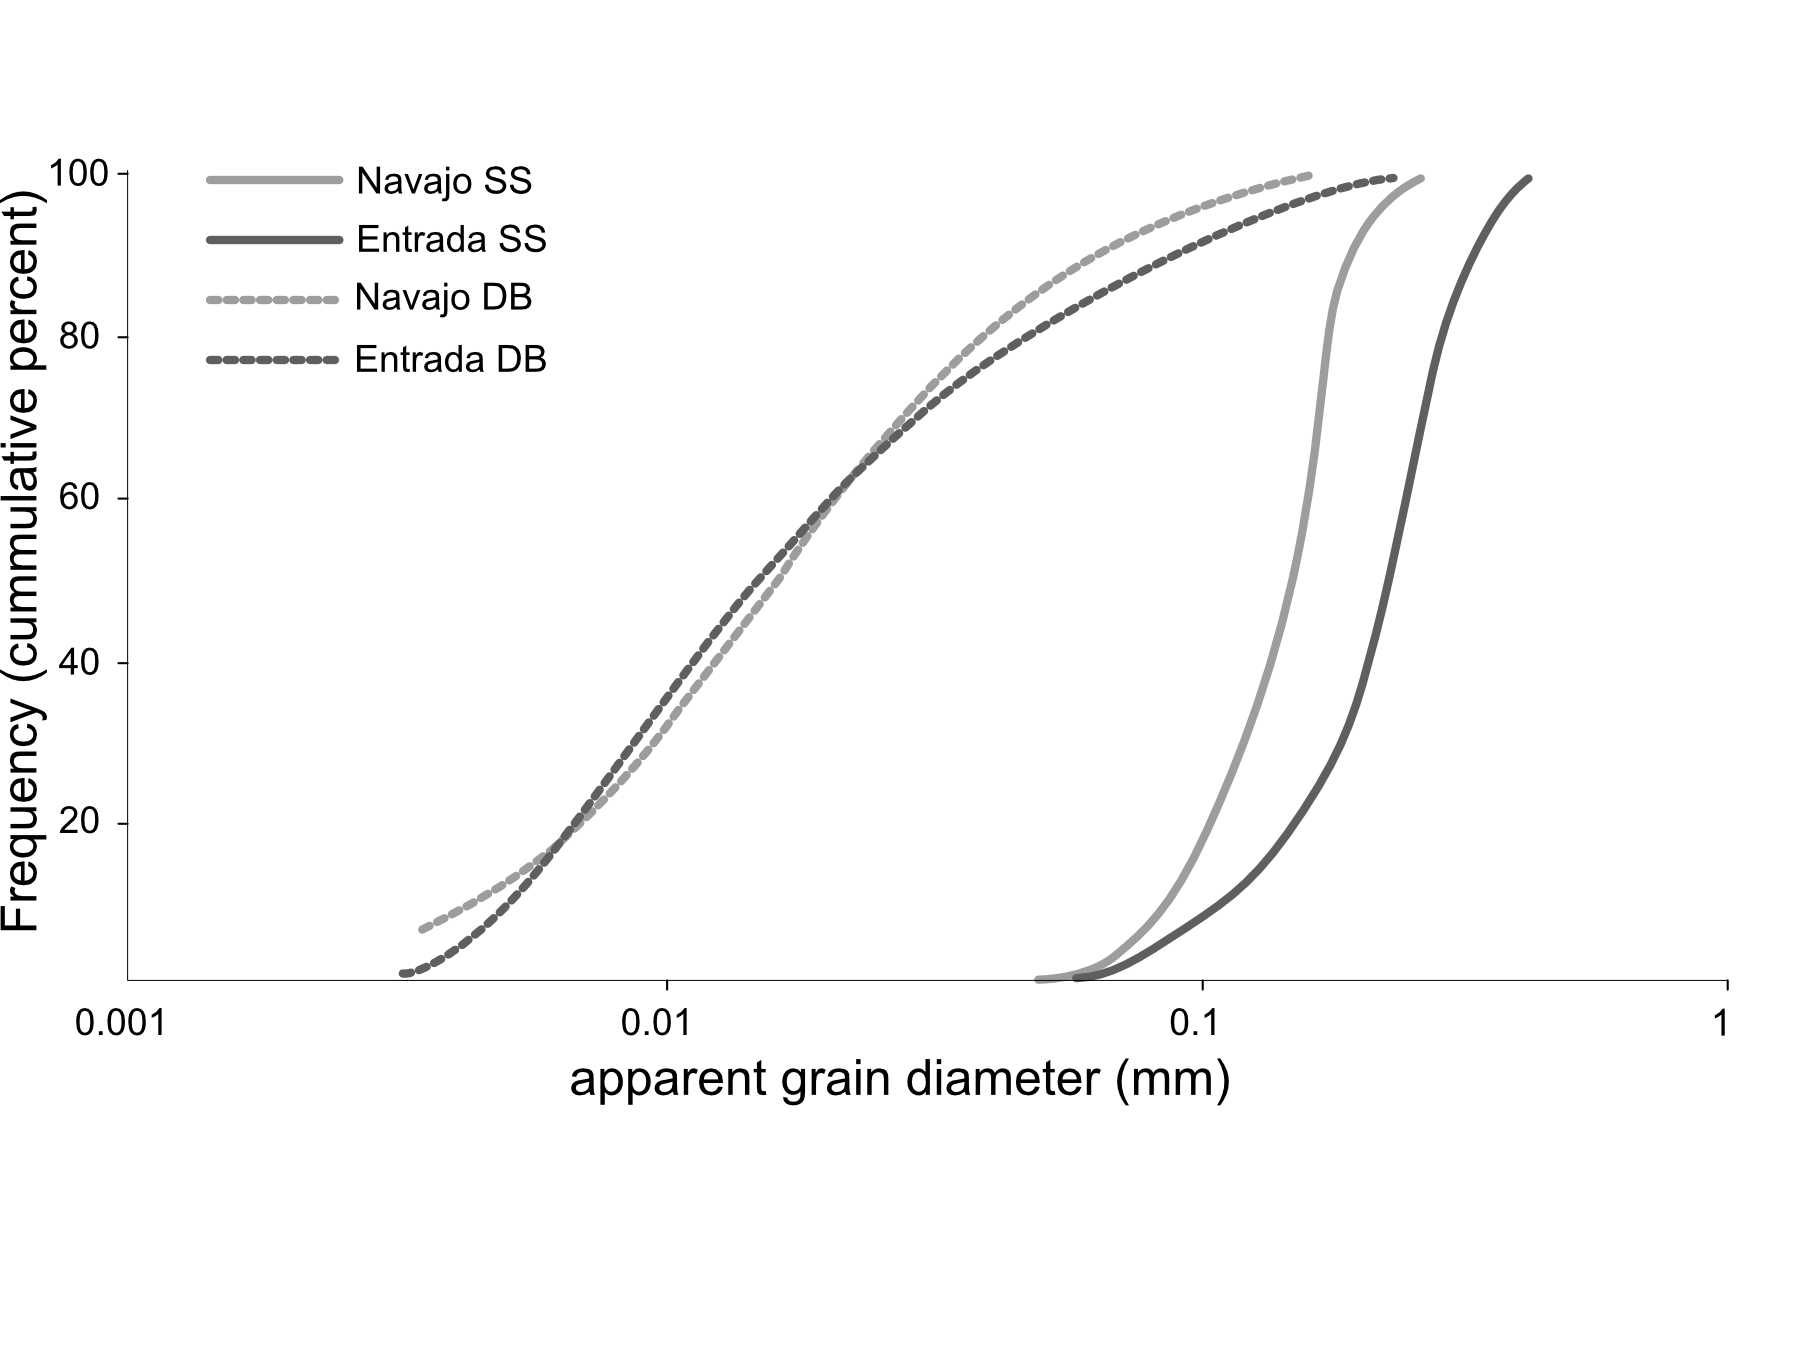
\includegraphics[width=\textwidth]{Grain_size_distribution}

	\caption{Grains size reduction of crushed grains within deformation bands relative to the underformed sandstone units, the Navajo and Entrada sanstones. (figure adapted from Aydin, 1978)}
	\label{grain_size}
\end{figure} 


\begin{figure}[h]
	\centering

		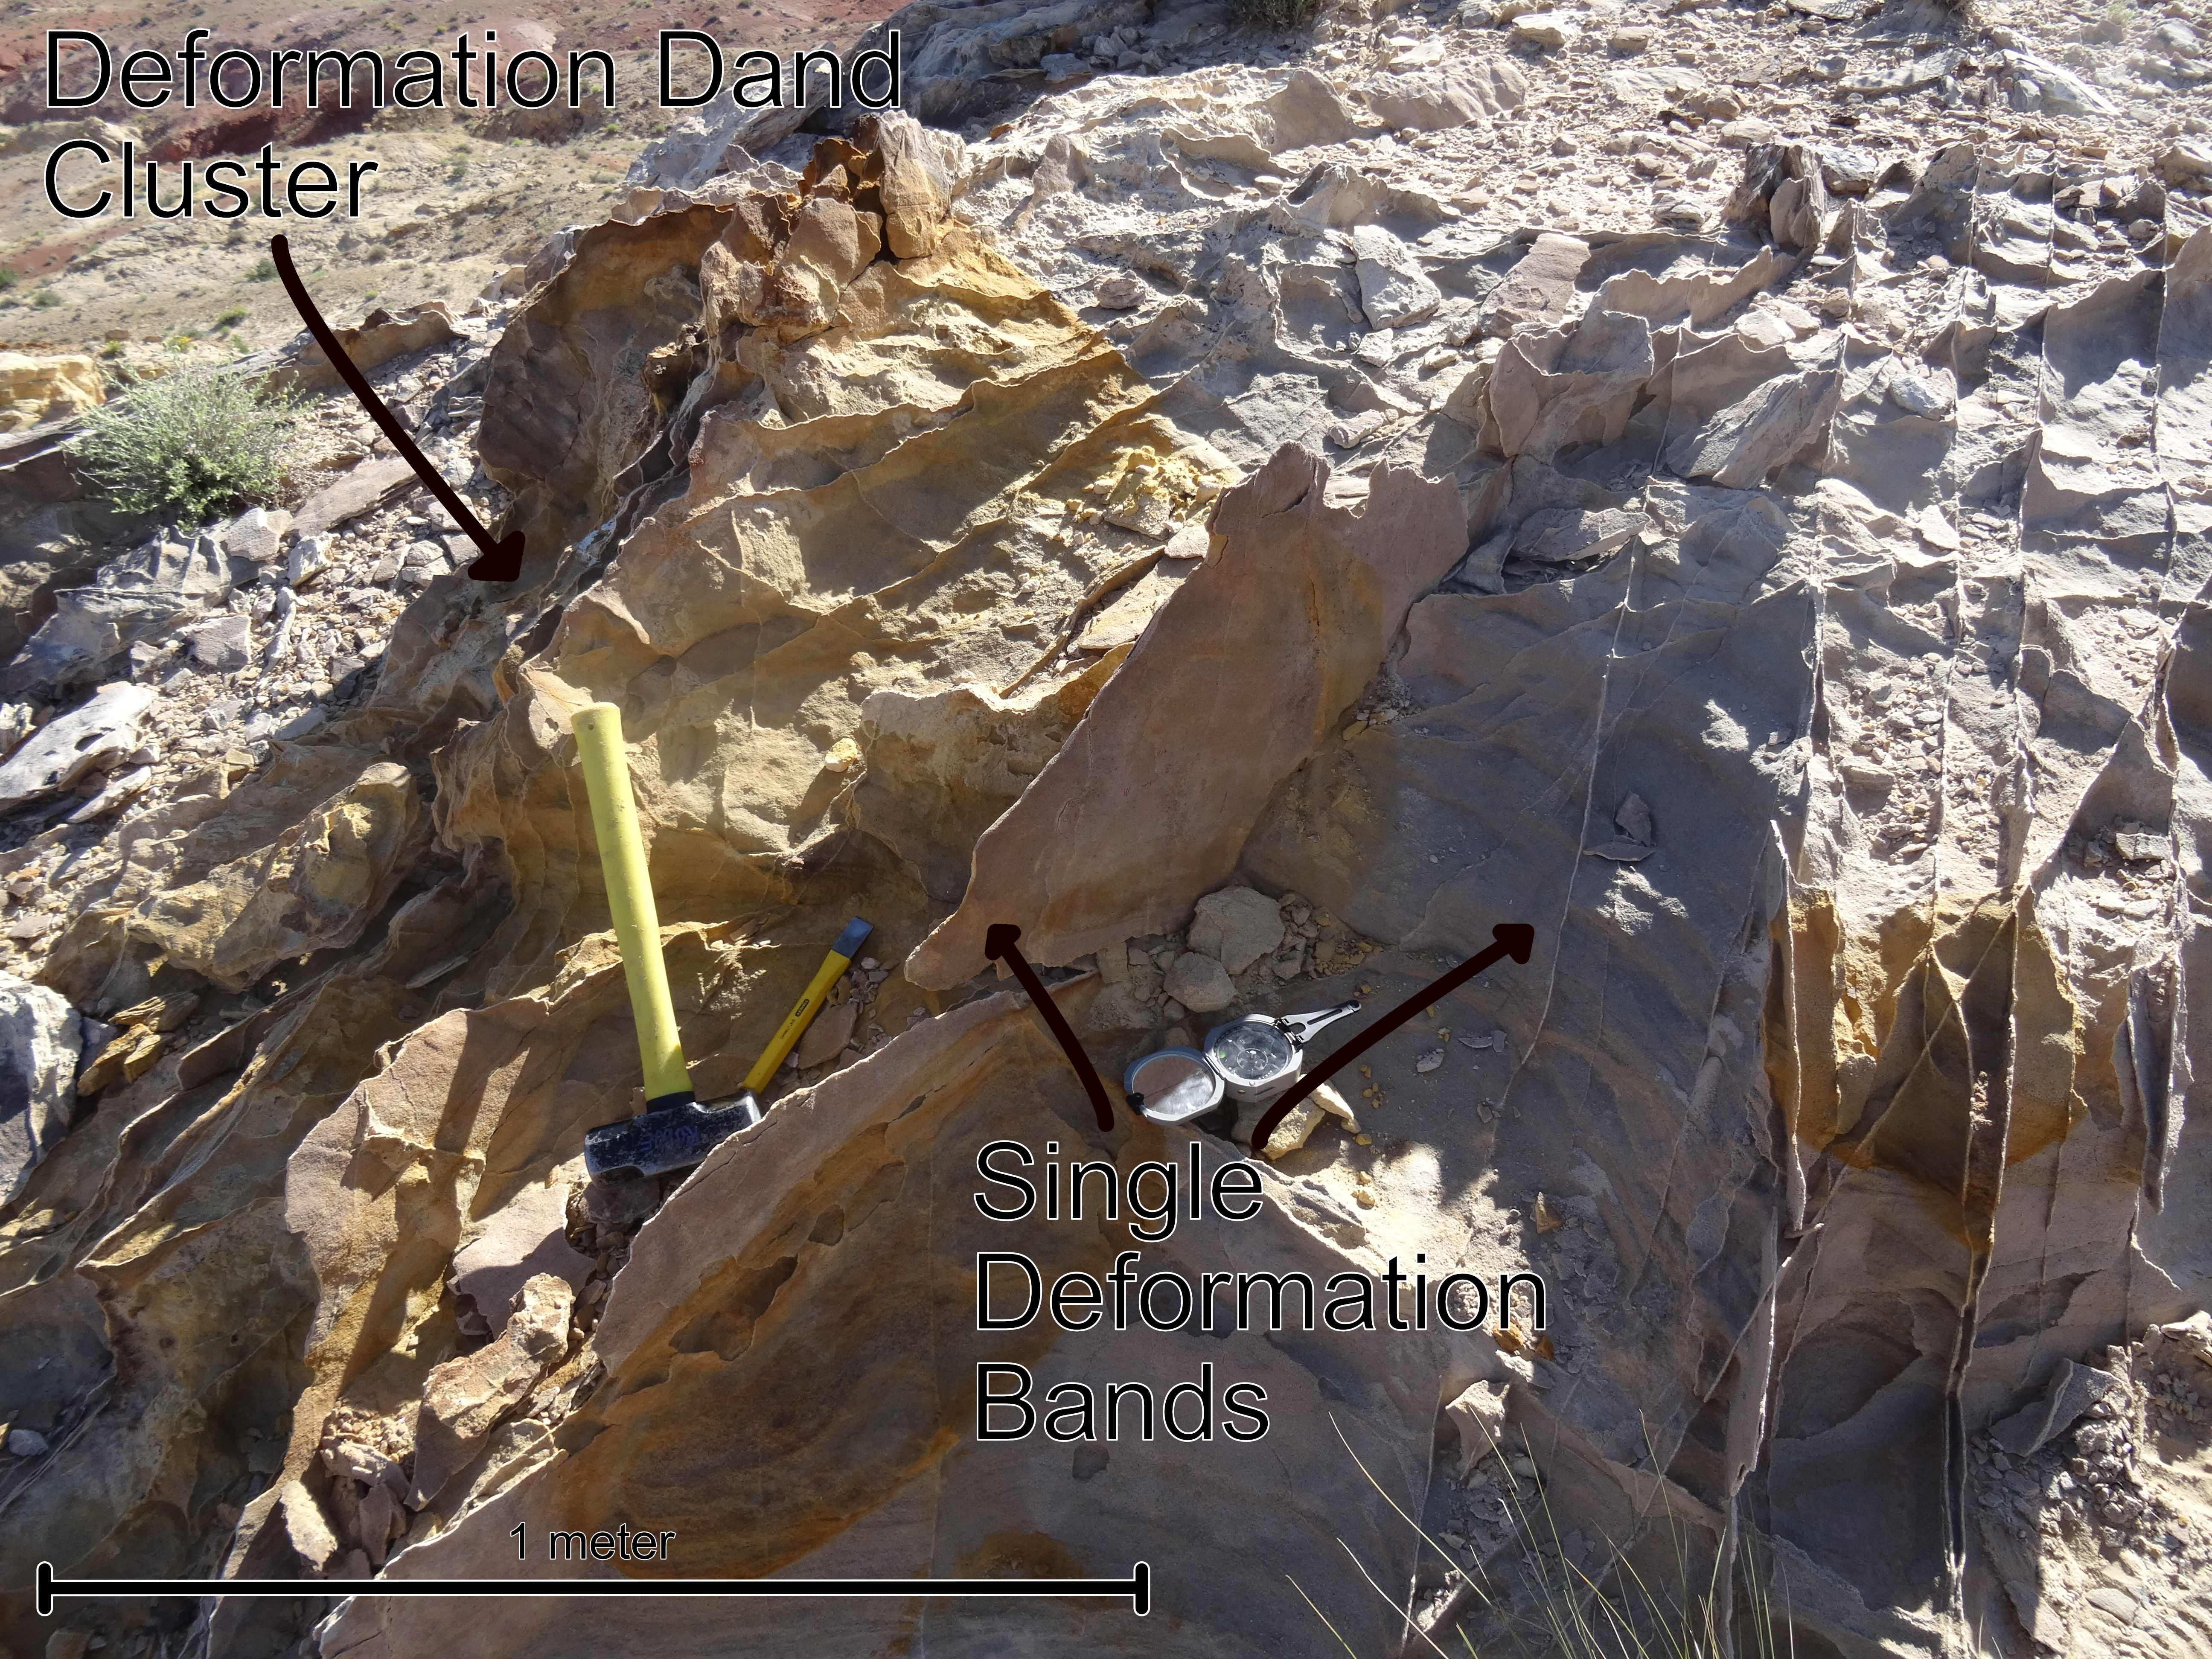
\includegraphics[width=\textwidth]{Defomation_Bands}

	\caption{Example of single deformation bands protruding out of outcrop. A small deformation band cluster is also visible in the background.}
	\label{deformation_band}
\end{figure} 

Deformation bands often outcrop as coalesced nearly co-planar groups or clusters. Deformation band cluster accommodate more intense and localized shear strain. Larger clusters often have one or many through going slip surfaces. The clusters are dense networks of anastamozing deformation bands ranging from a few millimetres to tens of centimetres in width, often outcropping as slabs up to meters in sizes. This erosional feature is most clearly expressed in the Entrada Sandstone. Clusters commonly form in upright conjugate pairs, each dipping around $~60^o$ in opposite directions.   

Edges of deformation band clusters that have eroded out appear to have distinctly corrugated and "lumpy" morphology (see figure \ref{DBC}-left). The orientation of the corrugations is in clear agreement with the kinematics of through-going slickensided slip surfaces. The slabs are coated with sand grains from the host sandstone. There is a clear directional asymmetry along the direction of shear whereby steep faces are in the direction of shear offset and shallowed faces are in the opposite directions (see figure \ref{DBC}). The asymmetry is observed on either side of deformation bands clusters. Refer to Fossen et al., 2007 and Aydin, 1978, for more detailed and very extensive characterizations of defomation bands in these localities.

Pre-existing regional joints sets are a common feature of every locality.  Joints typically have dips near $90^o$. Joints set are best defined in the upper Navajo units and low Carmel limestone pavements. The intensity of joint increases near the fault with the occurrence of syn-kinematic sheared and splay joints \cite{davatzes2003overprinting}. Refer to Aydin and Davatzes, 2003, for extensive analysis of joint characteristics and relative timing for each locality.

The Entrada unit has more deformation bands and fewer and less well defined joints. Moreover, in the Chimney Rock fault array, there is a clear association to the conjugate fault set orientation. Faults striking 

 \begin{figure}[H]
	\centering
	\begin{subfigure}[b]{0.4\textwidth}
		\includegraphics[width=\textwidth]{DBC_edge}
	\end{subfigure}
	~
	\begin{subfigure}[b]{0.4\textwidth}
		\includegraphics[width=\textwidth]{DBC_X}
	\end{subfigure}
	\caption{Left: Example of the edge of a deformation bands cluster at Molly's Castle. Note the "lumpy" morphology and an clear vertical directional asymmetry. Right: Cross-sectional view of a deformation band cluster with tens of centimeters of shear offset. It is unclear weather there is a through going slip surface localizing displacement. It is , however, definitely not on the edge of the cluster.}
	\label{DBC}
\end{figure}		


\subsubsection{Slip Surfaces}

Slip surfaces in the Navajo and Entrada sandstones are most readily identifiable by their vitreous polish. Striations and grooves on the slip surfaces mark the direction of slip. In Cross-section, slip surfaces are discrete, through-going and smooth relative to their zero-displacement counterparts. Thin layers, less than a few centimeters in thickness, of milky white layers bound typically bound the slip surface. The slip surfaces often cross-cut or bound deformation band clusters. For a given slip surface, perpendicular profiles are notably more sinuous than slip parallel profiles. Slip surfaces are only preserved in the Navajo and Entrada Sandstones. In spite of good exposures in prospecting pits and careful inspection of the slip zone, the Navajo-Carmel contact at the Chimney Rock fault array did not preserve good surfaces in the Carmel Unit. It is unclear whether this indicates that the Carmel units is more susceptible to erosion and/or alteration; or if a polished finish is only a feature of the quartzite sandstones. Pristine fault slip surfaces are not cohesive, and readily form a parting surface. Fresh slip surfaces uncovered \textit{in situ} reveal a relatively consistent meso-structure (see figure – figure similar to that in Jamies notes), A sharp interface, separated by a sub-mm thick layer of incohesive white powder bounded by two vitreous surfaces is a dense set of deformation bands. 

 \begin{figure}[h]
	\centering
		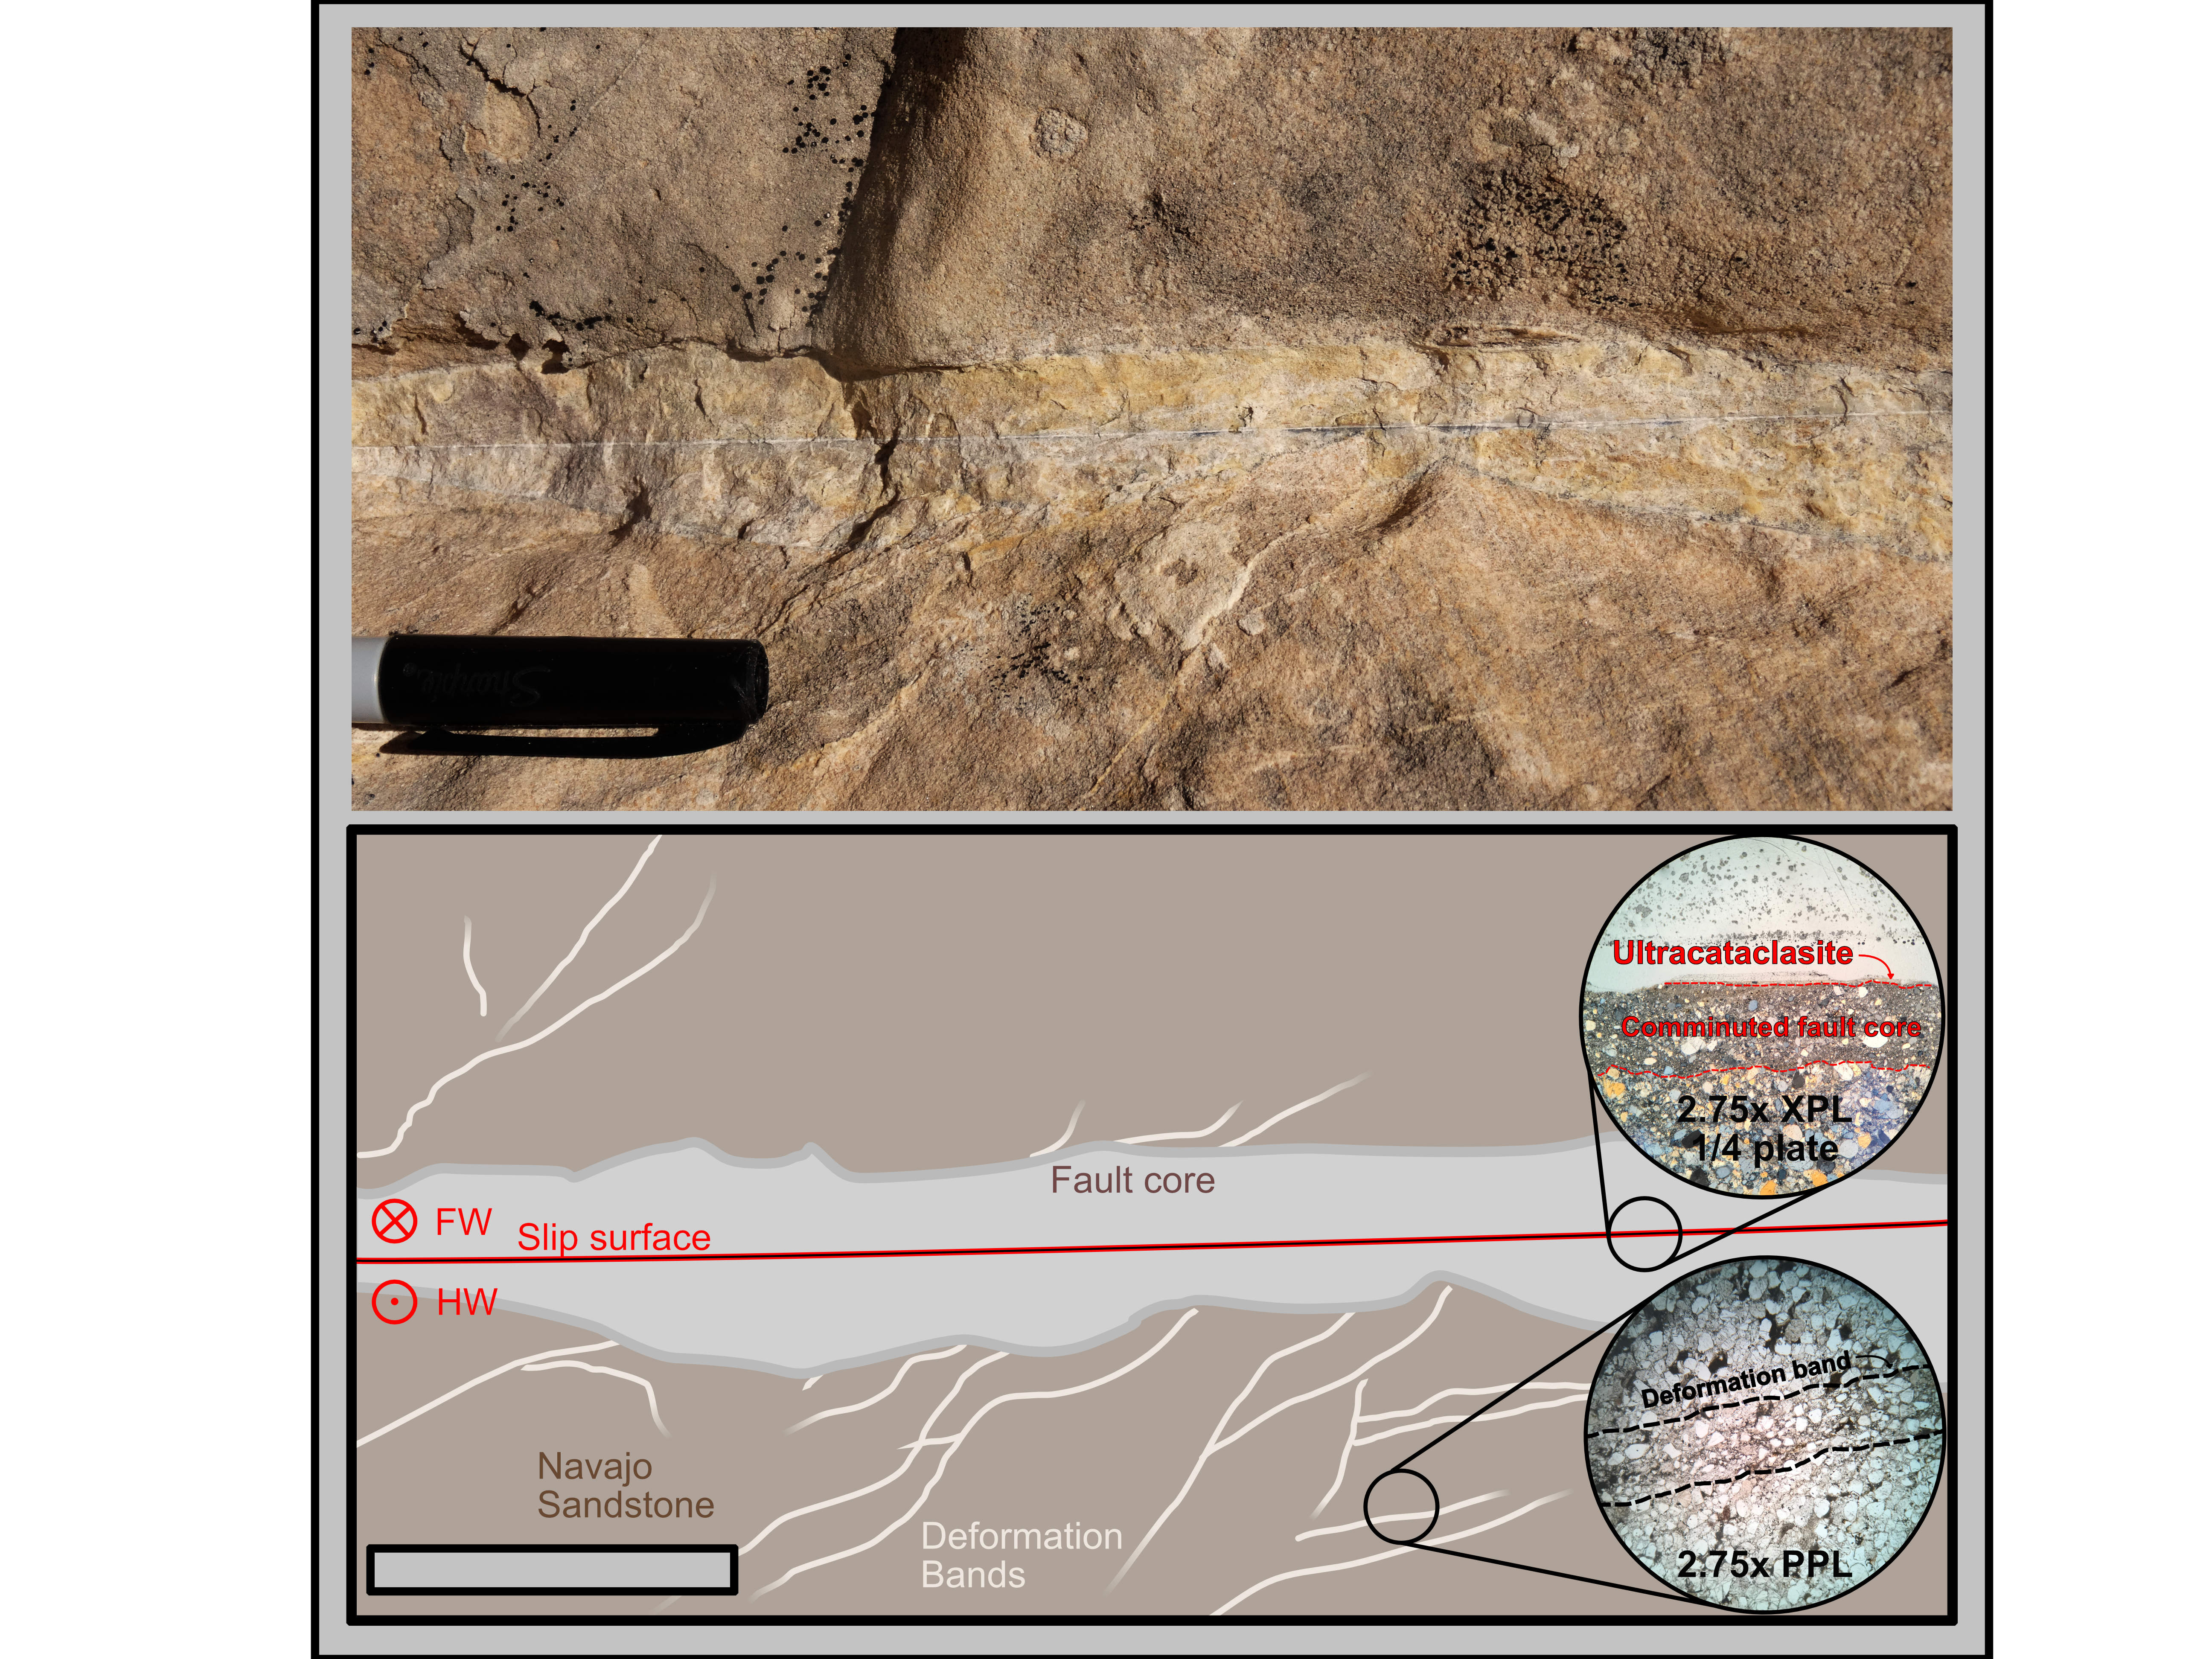
\includegraphics[width=1 \textwidth]{Fault_architecture_zoom}
	\caption{Top: Example of representative meso-structure of faults in the Navajo sandstone. Bottom: Cartoon of the representative meso-structure with slip surface (red), fault core (grey), deformation bands (pale beige) and intact host sand stone (brown). Upper half is the footwall; lower half is the hanging wall. Exposure is slip perpendicular. Representative thin sections show (not in situ) show the bottom half of the fault core (top) and deformation band (bottom). The section through the slip surface shows the microstructural architecture of slip surfaces with a very fine layer (barely visible) of ultra-cataclasite and a bounding comminuted layer. Note that this section is still well within the fault core. The section through the deformation bands shows the gradational reduction in grain size (outlined by black dashed line).}
	\label{DBC}
\end{figure}

In spite of careful preparation using epoxy, thin sections all parted at the slip surface interfaces. Moreover, samples only recording one side of the slip surfaces only partially preserved the edge of the slip surface.Thin section observations reveal a layered micro-structural architecture of the faults rock locally bound slip surfaces. The following succession, ordered according to distance from the slip surface is typical for slip surfaces in sand stone:  1) a very fine grained ultracataclatic layer, 2) a broader comminuted layer (sometimes absent) and 3) a deformation band zone which grades into the intact protolith.

The ultacataclasite is continous, nearly always bounds the slip surface, and ranges from sub-milimeter to 2 milimeters in thickness. Grain size distribution clearly has a steep fall off with most grains being unresolvable at 400 fold magnification. Larger grains are rounded to angular and do not exceed 10's of micron - significantly smaller than protolithic intact grains which are on the order of 100's of micron. Ultra-cataclasite layers show evidence of localized failure (see figure indicative of cycling between healing and brittle failure. Larger survivor grains within the layer are partially offset(see figure xxx). Ultra-cataclasite layers preserve a faint foliation oblique to the bounding intact rock. The kinamtics from the flow banding are consistent with sense of shear of grains protruding into the untra-cataclasite and partially sheared off. Previous work has shown no notable change in in the major elements, silicon, calcium, potassium and sodiu, of the undeformed sandstones  \cite{aydin1977faulting}.

The broader comminuted layer is not always present. Instead, the fault, still bounded by a thin ultra-cataclasite directly transitions into the intact host. When present, the comminuted layer is onset by a discontinuous interface with layer 1, the fine grained cataclasite. It is evidenced by a distinct change in grain size and spatial arrangement. Past this transition, grains are larger and preserve damaged but intact sedimentary textures from the sandstone. In contrast to the ultracataclasite, the original grain geometry is sometimes still discernible. Grains size within the comminuted layer is spatially variable with bands or lens' of larger grains separated by finer, more angular grains, texturally similar to deformation bands but showing more advanced stages of grain size reductions and shear localizations.

The textural transition is best explained  by dynamic grain size reduction and wear at the slip surface interface producing ultra-cataclasite which overprint more diffuse off-fault grain size reduction through grain crushing and deformation band production. This layer has highly variable thickness which typically ranges from millimetres to centimetres. Its thickness is asymmetric relative to the slip surface. Variability is directly associated to splay features which intensify mechanical damage around the fault.
Dark oxide filled fractures up to a few centimetres in length abut steeply into the slip surface and over-print other fault-related textural features. These are characteristically consistent with dynamics tensile cracks and would correspondingly be indicative of seismic rupture velocities.

Scattered Electron Microscopy (SEM) reveals 

Reddish-brown to dark tarnish and reduced vitreous lustres are indicative of advanced erosion. Sections of the slip surface are plucked off. Severely weathered scarps, not scanned in this study, develop a slip perpendicular fabric associated to conjugate fractures and deformation bands abutting into the slip surfaces.  In the Chimney Rock Fault Array, lichen grew preferentially on north facing scarps. From our field observation, it is clear that erosion has the effect of re-roughening the slip surfaces, especially at smaller scales. We can confidently attribute these re-roughening effects to erosion because they did not occur in freshly parted slip surfaces.

The evolution of slip surfaces with displacement is qualitatively apparent. Faults with small displacements (centimetres of offset) are distinctly different than larger displacement faults (meters of offset). They are 1) visibly more sinuous, 2) laterally discontinuous, 3) less polished, instead, having a dull lustre, and 4) not bounded by well-defined gouge or cataclasites layers bounding the slip surface visible in the field. In spite of extensive investigation, we do not observe faults with well-defined slip surfaces with clear offset markers indicating less than approximately half a centimetre of displacement. It is unclear whether this is the result of an undeveloped reductions in cohesion, as that associated to other slip surfaces observed in the field, or whether it is mechanically favorable to produce deformation bands at such low strain.

\begin{figure}
	\centering
	\begin{subfigure}[b]{0.4\textwidth}
		\includegraphics[width=\textwidth]{two_slip_surfaces}
	\end{subfigure}
	~
	\begin{subfigure}[b]{0.4\textwidth}
		\includegraphics[width=\textwidth]{Concentric}
	\end{subfigure}
	\caption{Left: Example of at least two distinct polished slip surfaces on the same fault structure. Right: Example of concentric pattern on cross-sectional view a fault}
	\label{many_surf}
\end{figure}	

\begin{figure}
	\centering
    \includegraphics[width=1\textwidth]{PSS}
	
	\caption{Example of a slip surface interpreted as a principle slip surface with around 20 meters of displacement at Big Hole Fault}
	\label{PSS}
\end{figure}

\subsubsection{Fault architecture}

Slickenline orientiation of faults in the Navajo and Entrada sandstones indicate normal dip slip with some instances of strike slip offset. Rotation of the slip-direction typically neighbours point of fault intersection \cite{davatzes2003overprinting} \cite{maerten2001digital}. Faults outcrop in relays and cross-cutting conjugate sets. We record dip angles ranging from $44^o$ to sub-vertical with an average dip angle of $70^o$. The single slip surface accommodating the bulk of stratigraphic offset is not systematically representative of the fault architecture. Often, fault zones instead have many slip surfaces, sheared joints and splays which partition offset. As is characteristic for high porosity sandstone \cite{aydin1978development}, fault zones all have deformation bands. The intensity of deformation bands rapidly decreases with increasing distance from the fault. according to a power law away from the center of the fault zone and was shown to correlate in intensity with displacement on the fault . Deformation bands typically abut obliquely into the slip surfaces at shallow angles (less than $70^o$).

Certain slip surfaces clearly accommodate the overwhelming majority of fault offset. Displacement accommodated by smaller neighbouring discontinuous slip surfaces is minimal (Shipton, XXX). Based on observations from previous workers and those made in this study where larger displacement slip surfaces are unambiguously identifiable allowed us to characteristically further its characteristics generalized for the Navajo and Entrada Sanstones as follows:

\begin{itemize}
	
	\item \textit{Large displacement faults are distinctly more discrete and planar}.
	
	\item \textit{Larger displacement faults are not cross-cut by deformation bands or more sinuous and discontinuous slip surfaces}
	
	\item \textit{in line with the implicit definition of a fault, the PSS is nearly cohesionless.} Locations identified to be expose section of a PSS inevitably cracked open when sampling across the slip surface--the slip surfaces had no cohesion. Cohesion is typically thought to reinstate by precipitation and healing. We did not observe recovered healing in this study.
	
	\item \textit{Large displacement faults have a vitreous finish};
	
	\item \textit{Large displacement slip surfaces are typically in the center of a damage zone}. Damage in an inevitable consequence of displacement and the accompanying mismatch that accumulates. Damage at the field locations in this study is expressed as comminution (\textit{e.g.} cataclasite and gouge), fragmentation (\textit{e.g.} breccia, splay joints) and shear deformation (specifically deformation bands).
	
\end{itemize}

 


In this study, we refer to \textit{fault rock} as rocks  associated to a fault (Snoke et al. 1998). We pay careful attention to the fault rock as it is inevitably coupled to the slip surface roughness and its maturation with cumulative displacement. The faults in our study area display a very diverse range in fault rock lithologies, ranging from fine-grained cataclasites to massive  bodies of breccias (up to meters of thickness). 

Fault rock consistently bounds slip surfaces--often asymmetrically. However, observations at the outcrop scale (10’s of meters) both along the strike and dip indicate that both the lithology and thickness of the fault rock are highly heterogeneous and are subject to large variability. These observations are consistent with more detailed fault architecture mapping conducted by Shipton et el., 2002.  

We do not observe a clear and tractable relation between fault slip surface displacement and faults rock thickness. This is big part a result of difficulties in defining a clear fault rock thickness criterion which well encapsulates the variety of faults rocks -- a challenge well highlighted in  (Shipton et al., 2006).

* this stuff is left over's from  editing and moving things around

Healed Gouges
-	the spot at big hole
-	iron wash (powder between the surface)
-	micro-structure
-	prospecting pit
-	typically on thinned sections of the fault rock (near the slip surface)
Cataclasites ….
-	big hole sample with slip surfaces on both sides of the cataclasite
-	micro-structure
-	
Breccias…
-	thick sections  of the 
Breccias occur lenses which range from cm’s to meters in thickness. Breccia clasts are typically poorly sorted and can be very coarse with clast up to ~10 cm in diameter. Clasts show indications for multiple generations of brecciation.


Thin Quarts lens
-	iron wash


Systematic associations between fault rock and fault structure exist. For instance, Davatzes et al., 2002 reports of a systematic association between the fault rock lithology and the orientation of the fault set. Namely, the orthorhombic fault set striking WNW has systematic association with fragmentation—fault breccias; conversely the ENE fault set rather has slip surfaces cutting through deformation band clusters (see figure \ref{fig:DavatzesFR}). This relation was speculated to be the result of contrasting genetic mechanism. The WNW set is the result of the reactivation of regional joints. In contrast the ENE fault set is the the result of clustering and anastamosing deformation bands acting as a catalysing agent to the formation of a faults.
In this study, we observe clear instance of lithological contacts being associated to brecciation (photo at iron wash where the top of the Navajo is brecciated and quickly reverts to a single fault strand. More over, large breccia bodies are clearly related to points where faults are cross-cutting each other at high obliquity as is often the case at the Chimney Rock fault array and 

Complicating factors:

Associations between brecciation and lithological contacts…

Associations between brecciation and cross cutting faults…

For an extensive review and description of the faults in the Navajo and Entrada sand stones refer to Aydin’s thesis. 


\subsection{Interpretation of field observations and roughness measurements}

Cross-cutting relationships reported bot in this study and in previous work on faults in the Navajo and Entrada units of the San-Rafael swell are particularly informative. Large displacement slip surfaces are not cross cut by deformation bands and more sinuous slip surfaces. However, large displacement slip surfaces do cross-cut clusters of deformation bands and more sinuous slip surfaces. This relationship is indicative of a clear evolution of the fault architecture by 1) localizing displacement and 2) smoothing out slip surfaces. 

Faults zones with larger offset are associated to larger damage zones and more slip surfaces. This is particularly telling fact when with the observation that small displacement slip surface do not cross cut larger displacement slip surfaces. 

The cross cutting relationship implies that either slip either smaller less continuous slip surfaces predate the onset of the larger offset slip surface or that the they splay off of it. However, we can reject the former as a possible mechanism as it does not account for the increased density of slip surfaces on larger offset fault zones.  This implies that they either form directly from the stress heterogeneities induced by the roughness of larger displacement slip surfaces. 

Slip surfaces pre-dating large The former case  stress heterogeneities from active slip surfaces induced by fault roughness.

%Observations from this study do not necessarily agree with this paradigm. deformation bands active after the onset of a stable slip surface \textit{have} been observed at Big Hole (Shipton and Cowie, 2003). Onset of late deformation bands may reconcile our observations with the existing paradigm for fault development in high porosity sandstones. We intend to explore the surface roughness of the edge of deformation band clusters. In a sense, these surfaces could represent a 'primordial roughness'.%

%At some locations, take for instance the Blueberry Fault in the Chimney Rock Fault Array, deformations bands seems to be the overwhelming mechanism to accommodate off-fault damage. When considering issues of fault mismatch related to roughness and consecutive displacement, deformation bands may be an effective mechanism to accommodate inelastic fault perpendicular deformation.%

faults are smoother than joints or deformation bands

At the grains scale, grains are truncated, not `plucked'.

more linear fault traces where not offset by wavier fault traces
	
\section{Geometric analysis}		

\subsection{Method}

This study focuses on the qualitative and quantitative evolution of fault slip surfaces—both addressing how fault slip surfaces evolve and the implications thereof. The quality of the displacement measurements and the large number of accurate surface scans are fundamental to the quantitative analysis of the data. Field-method and data acquisitions thus reflect these standards. 

For the qualitative analysis, we carefully record the characteristics of the fault architecture in the context of fault evolution. Specifically, we are particularly meticulous about 1) identifying cross-cutting relationships which indicate temporal evolution on the on fault, 2) identifying the evolutionary stages in the formation of faults and 3) identifying and characterizing the wear product, or fault rock, produce as faults evolve. 

For the quantitative analysis, we collect scans both \textit{in situ} and from hand samples collected in the field. Scans are associated to a constraint on displacement. Moreover, for every scan, the time of day, location, quality, strike and dip of the fault slip surface as well as the rake of the slickenlines are recorded. When possible we record an estimate of the fault rock thickness. Finally, we also record both a plan and cross-sectional view image of the scanned fault surfaces.  See appendix for the tabulation of this data. Together, all these measurements and observations should provide the necessary data to robustly explain and quantify the process through which faults mature.

	\subsubsection{Scan Data Acquisition}

To measure slip surface roughness, we analyses large point clouds scans of real fault surfaces and average the slip parallel and perpendicular spectral and statistical properties across hundreds of profiles. Point clouds must be obtained across a flexible array of instruments to properly capture the fractal scaling behavior (Brown and Scholtz, 1985; Candela et al., 2012). In this study, we use three instruments with complimentary scales of observation.  Together, these instruments offer accurate and precise three-dimensional discretization of fault surfaces at over nine decades of length scale.

*make a map of each areas with the location of every scan encoded with different symbols*

At the largest scales ranging from meters down to millimetres, a light detection and ranging instrument (i.e. LiDAR). We use the  LiDAR has been used in many previous studies of fault roughness as it is easily deployable in the field and provides rapid means to collet very large point cloud data set. However, its use is limiting as it requires exceptionally good and, accordingly, rare exposure of fault surfaces that are large enough and fresh enough to not have been degraded by erosion. In this study, we report 5 ??? Lidar Scans (see figure).

Instead, the bulk of in situ field measurements were made at intermediate scales ranging from centimeters down to hundreds of microns with the NextEngine 3D laser scanner. The NextEngine laser scanner is accurate down to 100 microns with resolution up to 41 540 points per square centimeter. Note that the NextEngine is a much less cost prohibitive option when compared to the LiDAR yet captures the same characters of the fault surfaces. The laser scanner was benchmarked to a machined-flat granite surface and to a scan of the corona slip surface both to industrial-grade laser scanner as reference. The scanner is not exactly built to be field ready. It requires a power source, low light conditions, a stable surface to sit on, limited dust exposure and must be connected to a computer. Moreover it only allows for a very limited depth of field. To use the scanner in the field, we connected both the laser scanner and laptop to a solar powered, \textit{goal zero}, battery. The scanner was encased and padded in a reinforced cardboard box with its depth exactly equivalent to the optimal depth of field. The set up had the added advantage of being very portable, completely removing sunlight and limiting dust exposure. We report XXX scans using the NextEngine Laser scanner.

Finally, hand samples were collected and analyzed with the Zygo blah blah, an optical profilometer enabling accuracy from milimeters down to sub-micron. The Zygo blah blah uses white light interferometry to produce relatively small point-clouds (XXX points) a various magnifications. It does however allow for seamless stitching of scans. Individual and stitched scans using the profilometer where benchmarked to a silicon carbide reference machined flat to XXX meters. All samples where scanned at 20x magnification and stitched together to produce sections roughly XXX by XXX millimeters. In additions, samples where scanned at the lowest magnification to properly bridge the gap up to the laser scanner resolution. We report scans of XXX samples with the white light profilometer, XXX of which were taken from surfaces scanned in the field with the laser scanner.

	\subsubsection{Constraining displacement}

We associate every scan with a displacement constraint. At The Chimney Rock Fault Array and Big Hole Fault entire displacement profiles have been measured during previous mapping campaigns (i.e. Maarten  shipton).  At Iron wash, Horse Creek and Molly’s Castle, Atilla Aydin’s mapping identified clear offset markers where available. Base maps for all field locations were georeferenced using satellite images when necessary and use as a reference in the field to streamline scan data acquisition. Displacement where estimated after the field campaing using GPS locations collected in the field. Additional measurements using basic tape measure and compass triangulation methods where also obtained in the field.  

Base maps only report stratigraphic throw or, in some cases, offset across \textit{entire} fault zones. However, many slip surfaces, complex networks of deformation bands and sheared joints which partition offset across fault fault zone (see figure). We therefore make a distinction between \textit{offset} across an entire fault and \textit{displacement} across a single slip surface. Without good marker horizons and cross-sectional exposure, stratigraphic offset is accommodated across slip surfaces is ambiguous. Offset across the entire fault zone therefore only serves as an upper-bound constraint on displacement across a single slip surface slip surface. In XXX of XXX fault slip surface measurements, this is the best available constraint on displacement. 

 PUT THIS UNDER FIGURE "At Big Hole fault, two large-scale continuous strands of the fault, both accommodating meters of displacement exemplify this mechanism at a larger scale. In accordance, Shipton and Cowie, 2003 report large uncertainty on the partitioning of stratigraphic offset across the two strands".

We were able to reconstruct exact displacement in the following specific cases: 1) If full cross sectional exposure indicates a single slip surface; 2) If cross-sectional exposure is good enough to clearly indicate an offset marker (lamella, cross-bedding or lithological contact) and its attitude, traceable to the slip surface exposure; or 3) if it is unambiguous that one principle slip surface is accommodating an overwhelming majority of fault offset, i.e. it is continuous, it has a layer of fault rock and unmistakably more linear and sharp than any other slip surface in the fault zone. 

Errors on displacement estimates are either reported directly for previous work (i.e. $1m$ precision for Maerten's throw measurements and $5m$ for Shipton's offset estimates) or conservative $10\%$ error on displacement estimates measurements made directly in the field. 

*make a table regarding the different types of displacement constraints*

known 		unknown 	equation 	assumptions		N

- throw - assuming 60 deg dip, dip slip 
- throw, dip – assuming dip slip 
- throw, dip, rake – assuming constant displacement orientation
- direct off-set – with different permutations …

	\subsubsection{Scan data Processing}

I use point cloud spatial statistics to characterize and quantify active surface processes on faults. I develloped a \textit{MatLab} work flow to entirely automate data processing from the raw \textit{.xyz} input fromat to the final statistical analysis:

\begin{enumerate}
	\item Preprocessing
	\begin{enumerate}
		\item manual inspection for coarsest defects
		\item Import \textit{.xyz} data into \textit{Matlab}
		\item Very coarse Height field filter
		\item Flatten points
		\item Grid data
		\item Orient grid along slip direction (using power spectral analysis 
		\item Remove defects
		\begin{enumerate}
			\item Remove outliers in the height field
			\item Fractal model filter
			\item Remove abnormally flat (interpolated) sections
		\end{enumerate}
	\end{enumerate}
	\item Processing
	\begin{enumerate}
		\item Statistical analysis
		\begin{enumerate}
			\item Scale dependent \textit{RMS}
			\item Scale dependent skewness
			\item Scale dependent kurtosis
			\item Scale dependent asymmetry
		\end{enumerate}
		\item Spectral Analysis
		\begin{enumerate}
			\item Fast Fourier Transform (FFT)
			\item Lomb-Scargle Periodogram
		\end{enumerate}
	\end{enumerate}
\end{enumerate}

\textcolor{red}{\textit{make into figure, include bypasses and other recent additions}}  

  
Note that the general pre-processing workflow was slightly adapted according to the different instruments that where used in the study. These adaptation were mostly attributable to the quality of the data at the various scales of acquisition and the actual instrument specifications. Scans collected with the LiDAR required more extensive manual point removal to avoid features such as vegetation, spurious outlier and large defects to affect the quality of the preprocessing. Scans collected at the intermediate scale with the laser scanner easily followed this workflow. Finally, scan collected with the white light interferometer did required minimal preprocessing and where aligned manually at the time of data collection. 

Before conducting a statistical analysis scan data must be pre-processed into a workable format. Scan data is a point cloud - a series of points with coordinates $x$, $y$ and $z$. Scans reported in this study typically have $10^6$ to $ 10^7$ points. In raw form, the point clouds are randomly oriented, noisy and still contain instrumental and physical artefacts. Physical artefacts include cracks, eroded sections, and vegetation; instrumental artefacts include noise, smoothing and scattering. All these features must be removed. The process of manual removal is labour intensive and unfeasible for a data set of the scope presented in this study. I rather opt to automate this process. Only very large defects (defects that may substantially effect the quality of finding a true mean plane) are manually removed.

The surface must first both be flattened and aligned along slip. Linear trends in the data induce an unwanted high frequency signal in data and also affect the quality of later interpolation onto a grid. Thus, $x$, $y$, $z$ data is rotated using around the axis $\textbf{u}$ as determined by the normalized cross product between the surface normal $\textbf{n}$ and a vector normal to a flat surface ($\textbf{n}_2 = [0 0 1]$): 

$$ \textbf{u} = {\textbf{n}\times\textbf{n}_2}/{|{\textbf{n}\times\textbf{n}_2}|} $$

with the rotation,

$$ R = \cos\theta\textbf{I} + \sin\theta[\textbf{u}]_x+(1-\cos\theta)\textbf{u}\otimes\textbf{u},$$

were $[\textbf{u}]_x$ is the cross product matrix of $u$ and $\otimes$ is the tensor product and $I$ is the identity matrix.

Fault surfaces are anisotropic. The direction of slip is preserved in the anisotropy whereby the 'smoothest' direction is slip parallel and the 'roughnest' direction is perpendicular to slip. The fault scan is rotated around the $z$ axis such that the direction of slip is along the $x$ axis. The direction of slip is by decimating raw data before iteratd steps of regridding, one-degree rotation and spectral analysis. In the radial search, roughness is quanified as the integral of the log-weighted power spectrum over the entire bandwidth of the sample surface. The angle associated to the minimum in roughness is then identified as the direction of slip and subsequently used to rotated the original flattened point cloud. The data is then interpolated onto a grid using a linear interpolation algorithm. The point spacing is automatically defined by the point density over the areal extent of the data:

\begin{equation}
	\Delta x = N_{pts}/A XXXXXX
\end{equation}

INCLUDE HISTOGRAMS FOR EACH FILTER


\textit{Defects} include all physical surface features that are clearly not associated any faulting process, \textit{e.g.} cracks, eroded patches, vegetation, etc.. Defects are idenetified and filtered out using combination of thresholding methods. These methods all revolve around identifying clear points or segments that are statistical outliers to the distribution characterizing the entire surface--abnormal points. 

The most aggressive filter implemented searches for outliers to the fractal model. The filter removes entire linear segments with abnormally high variance in the height field for the given scale of observation. For this implementation, I iterate over 10 filter scales. The scales are selected using a log spacing from the 10 points up to the length of the entire surface. The threshold for segment removal is chosen to be four standard deviations from the mean (should account for $<0.1$ percent of the data in a normal distribution). Note that, assuming a normal distribution of variance data for a given scale, the filter should not induce a systematic bias since the filtering is symmetric around the mean. However, surface features associated with a truly distinct mechanism of formation, in this case cracks and other defects that will typically have much higher variance, \textit{are} be removed. This general approach ensures that defects, regardless of their scale get identified and removed. This is important for any subsequent fractal analysis.

Abnormally flat sections arise as the result of triangular interpolation of sparse points. Typically, interpolation on the edge on a non-convex set of points is subject to this effect. These artefacts are readily identified in the curvature data. In the log-transformed absolute value curvature field, these sections appear to be nearly or exactly zero. The filter rejects point with curvatures less than $10^{-25}$. These values likely associated to the linear interpolation scheme.

Finally, all scan are inspected to make sure that the pre-processing was successful. The script fails to properly process scans that are excessively populated with surface defects. These scans were manually cleaned and oriented before re-processing them. Manual changes were executed in \textit{CloudCompare}. 

Pre-prossed scans are $N$ by $M$ scalar fields of fault surface topography(the sitance from the mean plane) aligned with slip along the $x$ axis. NaN values mark locations where data is missing or was removed by filters. Point spacing is defined the mean point density of the scan in the $x$-$y$ plane.

	\subsubsection{Statistical Analysis}
		

After pre-processing, scans discretize defect-free slip surfaces with grids with rows aligned with the slip direction. We compute the power spectral density content for every continuous segment of every single profile of the grid using a Fast Fourier Transform (FFT). Individual spectra are interpolated onto a master frequency vector. For a given frequency, the distribution of power values across the profiles through along the slip is strongly skewed (see figure xxx). The skewness is attributable to the non-negative constraint on power and residual outlying profiles (defects not properly removed). To provide a more representative and robust measure of maximum likelihood, we use the geometrical mean instead of the arithmetical mean. Accordingly, errors represent the 1$\sigma$ range in the log-transformed distribution. The analysis yields one representative spectrum for each scan.

The spatial frequency content of slip surfaces follow a power law. This characteristic is roughly fixed for a single slip surface regardless of the scale sampled in our instrumental array. Fixed scaling and its power law form in frequency space is a feature of the fractal character of fault surfaces. We can thus further distil the roughness measurements using the fractal model of the fault:

\begin{equation}
P(k) = Ck^{-\beta}
\end{equation}

Accordingly the entire spectral information of a scan can be summarized with the prefactor ($C$) and the scaling exponent ($\beta$). Determining fractal parameters from spectra is not trivial. \textit{A priori}, the fractal model is determined using a weighted power law regression through the spectra. Weights are determined according to the inverse 1$\sigma^2$ variance of the power estimates. However, confidence interval on the fit parameters are strongly sensitive to both instrumental and analytical biases (XXX schittbulh 1998). Biases induce unwanted high or low pass filters in the spectral content-amplifying or diminishing selective bandwidth. The combination of instruments and highly overlapping bandwidths provides a means to identify the affected sections and suppress methodological bias. The comparison of the power law fit through multiple heavily overlapping instrumental bandwidths to the representative spectral of individual scans highlights instrument-specific biases. In doing so, we identify conservative bounds on sections of frequency spectrum that deviated from the power law fit. For our instruments, we find that artefacts are particularly disruptive at the small scale instrumental limit. The LiDar and laser scanner are dominated by a shallower slope at the high frequency tail of the spectra which has been interpreted in previous studies as random noise (XXX). Conversely, the spectra of the scan collected using the white light interferometer have steeper high frequency tails. This artefact has not been reported in previous studies in spite of the extensive use of the instrument. This discrepancy is likely attributable to the comparatively limited and subdued use of aggressive smoothing filters both in the scan data and in the spectra our analysis. Affected bandwidths are omitted from subsequent analysis. In spite of this approach, small discrepancies in parametrization of the power law fit for a given slip surface render the extrapolation of measurements from on instrumental bandwidth to the other instrumental scale of limited use. We therefore choose to report any further results at the bandwidth or specific wavelength best captured by the instrumental magnification.
	

INCLUDE A FIGURE WITH: ORIGINAL SURFACE, AUTOMATICALLY PROCESSED GRID, MANUALLY PROCESSED GRID AND CORRESPONDING POWER SPECTRA.


identifying fractal scaling section
	plot of white light all magnifications
	computational scheme to select the good section
error on direct displacement estimates?

\subsection{Results}

	
\subsubsection{Roughness measurements}

figures to include:
\begin{itemize}
\item all spectra
\item increasing anisotropy (two surfaces) - polar plot

\end{itemize}

Figure XXX shows the all the PSD calculations obtained from the scans collected in this study. Consistent with previous work, we find that the PSD spectra over the entire bandwidth reported in this study generally follow a power law scaling (a linear relation in log-log space). This feature corresponds to the constant fractal scaling. The scaling exponent and pre-factors are calculated using linear least-squares fit of the spectra in log-log space. The Hurst exponent can then be obtained according to equation XXX.

In the slip perpendicular direction, Hurst exponents range from XXX to XXX, with an average value of 0.8ish; Prefactors range from  XXX to XXX with an average value of XXX. In the slip parallel direction, Hurst exponents range from XXX to XXX, with an average value of 0.8ish; Prefactors range from  XXX to XXX with an average value of XXX. Implicit to the pre-processing grid alignment, for any single scan the slip parallel direction is systematically smoother than the slip perpendicular direction indicating a clear surface anisotropy. The entire data set does however indicate an overlapping range in slip parallel and perpendicular directions. We also note that lower pre-factors are generally associated to lower Hurst exponents.

An evolution with displacement is weakly expressed in the spectral analysis but is cluttered and obscured by highly variable errors on displacements and roughness measurements. In order to highlight the effect of displacement on the surface roughness, we separate our scan data into two distinct populations. 1) Scan data with direct displacement constraint and 2) scan data associated to maximum displacement constrains.  Brodsky et al., 2011, tested the validity of a power law relation between fault roughness are various specific scales and displacement. Building upon this approach, we use both data populations to test the validity and parametrization of the fit and the Implicit hypothesis that faults smooth as a function of displacement--the smoothing model. Scan data with direct displacement constraints serves as a direct test and a means to parametrize the smoothing model. For the model to be valid it must agree with further constraints imposed by data with only maximum displacement estimates.

A point defined by the maximum error bound on displacement and the roughness of the fault surface is in agreement with smoothing model if it is rougher that roughness prescribed by the model as parametrized by direct measurement. Conversely, if the point is rougher that the model prediction, it is not physically possible in the model construct. A null hypothesis would prescribe no bound on the roughness and would simply have the predicted roughness of a fault be defined by the probability distribution function of the entire roughness dataset.

* probably will revisit this *

Accordingly, we can roughly estimate the probability that our distribution of data relative to the smoothing model is a random element of chance according to:

\begin{equation}
 P = \prod p(y_i>Y(x_i))
\end{equation} 
 
 
----------------------

Figures XXX to XXX shows the relation between roughness and displacement as interpolated a various scales of observation. Vertical error bars on the power spectral density are obtained from the confidence interval of the of the fractal model regression. Horizontal errorbars on displacement are defined on a case by case basis from field observations and previous work in on the fault arrays. We present both the fit through the our entire dataset (comprised of direct and upper bound constraints on displacement) and through the the directly constrained displacement estimates. Fits are obtained using a least squares linear regression through the log-transformed data sets. In order to provide error bounds on the fit parameters, we use a full Monte Carlo simulation sampling direct displacement estimated as Gaussian distributions, upper bound displacement constrains as completely random distributions across the entire possible range of displacements and power spectral density estimates as log normal distributions. Errors represent on standard deviation estimated from 10000 simulations.

The weak trend across the entire dataset imply and expectation of smoother slip surfaces in fault zones which have accommodated larger displacement. 

Conversely the stronger trend across the well constrained data implies that an individual slip surface smooths with displacement. The smoothing exponent varies according to the different scales of observation (XXX at the laser at the centimeter scale, XXX at the milimeter scale and XXX at the micron scale).  While a power law fit to the best constrained measurements is has poor fit metrics, we find a nearly perfect agreement with roughness measurements only associated to upper bound constraints.


Two constraints on displacement – two data populations
plot of all the spectra color coded with displacement
smoothing plots:
	parallel -> all scales
	perpendicular -> all scales
	Hurst exponent -> all scales
Fit for smoothing through direct data, discuss consistency with max disp data
Other statistical metrics?
	Poly-gausian features in the surface roughness
	Skewness of height field as a function of scale
		Null result worth reporting?
		Do a plot of the evolution of skewness at the grain scale?




qualitative illustration of maturity


\subsection{Hard facts}

The following is a list of  `hard facts' that can be established from the both the qualitative and quantitative data:

\begin{itemize}
\item faults are smoother than joints or deformation bands
	\begin{itemize}
		\item power spectrum shows that fault slip surfaces are systematically smoother that joint and deformation band surfaces  at all wave lengths reported in this study ($10^-6$ to $10^5$ meters)
	\end{itemize}
\item At the grains scale, grains are truncated, not `plucked'.
\item The roughness of a slip surface is sensitive to its displacement history. This result is robust across multiple faults both nucleated from deformation bands and joints and variations in fault rock and host rock lithology.
\item The smoothing exponent is likely more than 1 at certain scales - quote from Emily: ``In all of these cases, the scatter of the data is large, but the basic result holds: the absolute value of the exponent is much less than 1.''
\item The smoothing rate is highest at small displacements and decreases with displacement.
\item Smoothing occurs at all scales of this study
\item a slip surface from a large offset fault is more likely to be smoother
\item for any given the displacement on a fault, the smoothest slip surface roughly follows the same smoothing trend as that defined by direct displacement measurements. 
\item The roughness varies spatially on a slip surface - the scatter in the data exceeds the instrumental error
\item the height distribution of points on a slip surface can be far from normally distributed.
\item the Hurst exponent has a very large range in values (less than Zero to ~0.9)
\item more linear fault traces where not offset by wavier fault traces

\end{itemize}

\section{Model}

	In this study, we utilize work minimization and boundary element numerical modelling to capture the growth of fault damage and the effect of rough asperities. The modelling component is motivated by the following questions: can geometrical asperities fail through shear? In so doing, how do they fail?--and what are its sensitivities to asperity geometry and strength? Does strength heterogeneity and mechanical wear by the truncation of asperities properly capture the evolution of fault slip surfaces with displacement. These questions prompt the need for physically robust models that can be accomodating of complex fault or asperity geometries. The complexity of these geometries imply that off fault damage will grow in complex stress conditions-- conditions that are currently poorly captured by simple analytical solutions (e.g. \cite{chester2000stress}). Moreover, complexities related to the discontinuous nature of fracture are more simply captured by boundary element modelling than existing finite element of finite difference models. This simplicity arises from need of fewer, less sparse, sets of equations to solve (\cite{crouch1982boundary}). Limitations of the boundary elements approach for fault modelling and off fault damage predictions is the difficulty of accumulating offset. Maximum allowable offset is roughly half the length of boundary elements. Along with this complications is the implicit trade off between model resolution and displacement. Approaches can be taken to circumvent the challenge however its development and implementation are beyond the current scope of this study. 
	
	The model builds off of fric2D and growth by optimization of work (GROW) develloped by Michele Cooke and Jessica McBeck. Fric2D solves for displacement and stress conditions on fault elements with prescribed constitutive behaviours given prescribed boundary element stress boundary conditions and material properties in two dimensions. Constitutive behaviour of fault elements are defined by its static and dynamic friction, critical slip distance, and shear and normal stiffness. In turn the behaviour of the medium fault elements and boundary elelements is linear elastic defined by Poisson's ratio and Yougn's modulus. For its part, GROW predicts fracture propagation paths. It does so by minimizing the external work on a system. As a natural analogue, the external work is the tectonic work imposed on a fault and its fault blocks, together comprising the system. The model allows for the simultaneous growth of multiple fractures. The general algorithm uses the same boundary element method as fric2D to describe the fractures--linear dislocation elements that discretize the entire length of the fault. As a crack grows, dislocation elements are added radially to the tip of the crack so as to minimize the external work on the system normalized by the crack area ($W_{ext}/\Delta A$). External work is further defined as:
		\begin{equation}
		W_{ext} = \oiint (\tau u_s + \sigma_n u_n))dB
		\end{equation}
		
External work is readily calculated from the the output of fric2D. Accordingly it is possible to iteratively test a range of directions of growth, compared the external work required, and choose the energetically preferred direction of crack growth. This process continues until stress at the tip of the cracks is not sufficient to overcome the fracture toughness. Therein lies the general algorithm of GROW. 

In practice GROW utilizes almost the same inputs as fric2D. The user must specify what points are considered to be 'flaws'. Only the coordinates associated to the flaws are analysed and allowed to grow according to the GROW algorithm. The computational cost of multiple initiation points is large. Every added flaw grows the computational cost exponentially according to the angular range and resolution. We rather use fric2D to educate the choice of coordinated for the flaws on the fault. 

Stress conditions are assessed along the fault elements. Normal ($\sigma_{11}$), shear ($\sigma_{12} = \sigma_{21}$) and tangential ($\sigma_22$) stresses on the fault elements yield the two dimensional stress tensor. Its Eigenvalues in turn allow for the determinations of principle stresses ($\sigma_1$ and $\sigma_3$). These in turn allow for calculation of the Mohr Coulomb stress and the assessment of elements prone to failure in shear according to host rocks angle of internal friction ($\phi$) and cohesion ($c$).

\begin{equation}
\tau_m = \sigma_m \sin(\phi) + c \cos(\phi)
\end{equation}
%
where,

\begin{equation}
\tau_m = \dfrac{\sigma_1-\sigma_3}{2}
\end{equation}
%
and,
\begin{equation}
\sigma_m = \dfrac{\sigma_1+\sigma_3}{2}.
\end{equation}

We also assess element that may fail in tension. Elements with least principle stress in tension exceeding the cohesive strength of the medium are also identified as being prone to fail. In the likely case that entire fault segments (multiple fault elements) are in stress conditions exceeding the failure criterion of the rock, we choose local maxima of Coulomb stress and tensile stress along these segments as the failure points.

This additional functionality is implemented in Matlab an seamlessly links fric2d, failure assessments and GROW into one single workflow.

	\subsection{Model Results}

\section{Discussion}
	\subsubsection{Tying the model together with roughness measurements and model}
wear rate (character), tying together model with 



	\subsection{An external estimate of gouge production and fault thickness * this section will likely be removed}

The data collected in this study offers the unique opportunity to provide new indirect estimates of fault rock production, fault thickness and dilation rate over an entire fault. We know that 1) the primordial roughness is systematically rougher than mature faults, 2) the primordial roughness is relatively constant, and 3) the roughness can be estimated for a given displacement. Using these results, I will estimate the volume of fault rock produced through wear and the corresponding roughness induced accomodation space in the fault system.

Displacing two rough fractal surface in shear requires dilation. The expectation dilation can be estimated according to the amplitude of the largest wavelength ($\lambda$) being offset (see figure XXX). For a given displacement, $u$, the largest wavelength in the system will be $\lambda = 2u_i$. Using a fractal paradigm to define the average amplitude of a given wavelength according to the pre-factor $\beta$ and the Hurst scaling exponent, $H$, (*reference the equation*) we find that the dilation, $A$ can be expressed as a function of displacement:

\begin{equation}
	A(u) = \sqrt{\beta 2u^{-2H-1}}
\end{equation}

If we apply this to an entire fault system with displacement field, $U$, we can estimate the void space that would be produced:

\begin{equation}
	V_{void}(U) = \int_S \sqrt{\beta 2U^{-2H-1}}dS
\end{equation}

Since the fault system is closed any change in fault roughness $must$ be coupled to the fault core. If all changes in the fault surface are associated to a production of fault rock, we can effectively estimate the volume of fault rock that has been produced from diplacement $u_0$ to $u_f$ by comparing the volume integral under the corresponding initial and final slip surfaces $S(u_0)$ and $S(u_f)$.

\begin{equation}
	\dfrac {\Delta V_{fault rock}}{\Delta u} = \int_S S(u_0) - S(u_f) dS
\end{equation}

volume integral under the surfaces, $S$, can be estimated numerically according to the frequency distribution prescribed by the RMS the  entire fault system. Note that the RMS is estimated at the length scale of the entire fault; wear processes are active at all length scales below this.

\begin{equation}
	\int S dS \approx 
\end{equation}

Now for the displacement field, $U$, we can estimate the total fault rock produced by using the primordial surface roughness, $S(0)$, and the prediction of the surface roughness extrapolated to the length of the fault (* reference the the equation of smoothing *) such that:

\begin{equation}
	V_{fault rock}(U) = \int_S S(0)-S(U)dS
\end{equation}

The comparison between the two quatities is telling. If the amount of fault rock is

\section{conclusion}
	\subsection{future work}


\bibliography{Thesis_draft}
\bibliographystyle{plain}

\section{Appendix}

\subsection{Surface Processing scripts}

Or possibly a link to a git repository...

\subsection{User manual for script}

\chardef\_=`_

This manual should serve as both a basic guide to the logic and usage of the \textit{surface processing package}. 

The master function of the package is \textit{surfaceprocessing}. This function effectively deal with the inputs and direct computations towards the necessary functions. Outputs of the function are a .mat workspace file for each input data file. The workspace includes a structure (called \textit{parameters}) with the raw surface analysis outputs, the point spacing, the decimation factor (if any), the file name and the date of the analysis. The workspace also includes the grid form of the original inputed surface (called \textit{surface}), and the pre-processed copy that was used for the subsequent analysis (called \textit{zGrid}).  Inputs are always included in pairs. The former defines the type of input, the latter qualifies or quantifies the input. This structure allows for adaptability of the code to various needs. Options include the following:

\begin{itemize}
\item \textit{what to do?}: 'toDo', followed by the desired analyses on of: 'FFT','PLOMB', 'parameters' or 'all' (default is 'all') - can be a cell array. This specifies what kind of spatial analysis will be done on the input surface data. The spatial analysis is calculated and averaged across every single profiles along the surface.  The analyses are the following:
	\begin{itemize}
	\item 'FFT', a power spectrum computed using a Fast Fourier Transform (FFT) algorithm; 
	\item 'PLOMB', a power spectrum computed using a least-squares Lomb-Scargle algorithm;
	\item 'paramters', the calculation (as a function of scale) of the Root Mean Squared (RMS), skewness, kurtosis and asymmetry averaged across all segments of a given length on all profiles of the surface.
	\end{itemize}

'all' simply performs all the analyses outlined above.

\item \textit{skip pre-processing?}: 'bypass', followed by 'zygo', 'pre-processing' or 'no' to  be used input is already in aligned clean grid form - input files are then (default is 'no'). 'zygo' is specifically adapted to the proprietary data format of the white light in Wong. 'pre-processing' simply skips any pre-processing. This option requires a .mat structure with a field named 'grid' with the topography and a field name 'pointSpacing' specifying the point spacing (in meters). In either case the topography must be aligned such that the positive x direction is the parallel direction.	

\item \textit{for the parameter analysis, how many scales?} 'numberOfScales' followed by the desired number of analysed scales. This option is relevant to the parameters analysis. Note that this has a lot of effect on the amount of processing time (default is 10).

\item \textit{decimation}: 'decimationFactor' followed by the desired decimation factor (default is 1). Decimation is a useful tool to reduce computation time. The surface grid is sub-sampled according to the decimation such that a decimation factor of $k$ would imply that only every $kth$ point on the every $kth$ will be considered for hte subsequent analysis.

\item \textit{Instrument specific analysis} 'instrument' followed by 'white light', 'laser scanner' or 'lidar' (default does not set any instrument specific adjustments). Some instrument specific pre-processing steps are taken. Please contact me if you intend to use this as they may be highly dependent on the specific instrument used.
	 
\end{itemize}

For instance, \textit{surfaceprocessing('todo','FFT','bypass','zygo')} will only perform a power spectral density analysis and will skip preprocessing and assume that all input will be in the 'zygo' export .xyz format.

When the command is executed, the user will be prompted to navigate to the directory where the input data is located. IMPORTANT: the directory must \textit{only} contain files of one data format. There cannot be other files or sub-directories in the directory. The user will then be prompted to choose a destination for the output data. The requirements for the output location are less stringent. However, it is advisable to choose an empty directory such as to facilitate subsequent steps.

The next step is to visualize the output of the analysis. This is done using the \textit{unpack parameters} function. This function provides various visualization options for all files in the directory chosen by the user. The first input (the \textit{desired plot}) can be one of the following:

\begin{itemize}
\item[] \textit{'FFT'}: plot all power spectra;
\item[] \textit{'PLOMB'}: periodogram plot as determined by the Lomb-Scargle least squares analysis;
\item[] \textit{'topostd'}: plot of the root mean squared (RMS) as a function of scale;
\item[] \textit{'topoSkew'}: plot of skewness of height fields as a function of segment scale;
\item[] \textit{'topoKurt'}: plot of the the kurtoisis of height fields as a function of segment scale;
\item[] \textit{'PowerVsDisp'}: plot of power interpolated at a given scale as a function of displacement;
\item[] \textit{'RMSVsDisp'}: model RMS at a given scale as a function of displacement
\item[] 'Grids': shows both the original and pre-processed grid for the specified file 'fileName';
\item[] \textit{'Best Fits'}: best logarithmic fits to power spectra obtained from the fast fourrier transform analysis.
\end{itemize}

The functionality of the packages is broadly divided into three sections: 1) importing and preprocessing data, 2) performing various spatial statistics on the pre-processed data, and 3) unpacking the analysis output into figures.

In order to run smoothly the all functions included in the package should be kept in the same directory or on an accessible path. 

For reference, here is a quick outline of what each function does:

\begin{itemize}
	\item[] \textit{affine\_fit}: (from mathworks) Computes the plane of best fit using least squares normal distance;
	\item[] \textit{align\_grid}: finds the smoothest directions in a grid using FFT spectra and rotates and re-grids the input grid;
	\item[] \textit{fault\_spectral\_density\_simple}: Calculates the average lomb-scargle spectral density every row of a N by M array;
	\item[] \textit{FindErr\_loop\_anisotropy}
	\item[] \textit{flatten\_XYZ}: removes planar trends from XYZ data by applying a rotations matrix according to the best fit plane (affine\_fit);
	\item[] \textit{fractal\_model\_outlier}: Removes outlying segments according to a near-gaussian model for the distribution of RMS values at specified segment lengths (or scales);
	\item[] \textit{frequency\_spectrum}:Calculates the average lomb-scargle spectral density of all continuous 	segments on every single row of a N by M array;
	\item[] \textit{parse\_zygo\_format}: extracts the both the point spacing and topographic grid from the exported zygo format. Can also remove planar trend from data (substracted from grid);
	\item[] \textit{rotateZ}: applies rotation matrix on XYZ data
	\item[] \textit{surface\_analysis}: Aggregates the analysis functions and applies them to an input grid
	\item[] \textit{surface\_cleaning}: removes outliers associated to surface defects
	\item[] surface\_parameters: calculates spatial statistics and parameters along segments as a function of scale (RMS, skewness, directional asymmetry and kurtosis)
	\item[] \textit{surface\_preprocessing\_2}: deals with preprocessing input data (import data, cleaning and gridding data)
\end{itemize}


\end{document}

